\documentclass[12pt,oneside]{book}

%%%%%%%%%%%%%%%%%%%%%%%%%%%%%%%%%%%%%%%%%%%%%%%%%%%%%%%%%%%%%%%%%%%%%%%%%%%%%%%%%%%%%%%%%%%%%%%%%%%
%                                                                                                 %
% The mathematical style of these documents follows                                               %
%                                                                                                 %
% A. Thompson and B.N. Taylor. The NIST Guide for the Use of the International System of Units.   %
%    NIST Special Publication 881, 2008.                                                          %
%                                                                                                 %
% http://www.nist.gov/pml/pubs/sp811/index.cfm                                                    %
%                                                                                                 %
%%%%%%%%%%%%%%%%%%%%%%%%%%%%%%%%%%%%%%%%%%%%%%%%%%%%%%%%%%%%%%%%%%%%%%%%%%%%%%%%%%%%%%%%%%%%%%%%%%%

% $Date: 2013-11-26 10:43:59 -0500 (Tue, 26 Nov 2013) $
% $Revision: 17538 $
% $Author: gforney $

%%%%%%%%%%%%%%%%%%%%%%%%%%%%%%%%%%%%%%%%%%%%%%%%%%%%%%%%%%%%%%%%%%%%%%%%%%%%%%%%%%%%%%%%%%%%%%%%%%%
%                                                                                                 %
% The mathematical style of these documents follows                                               %
%                                                                                                 %
% A. Thompson and B.N. Taylor. The NIST Guide for the Use of the International System of Units.   %
%    NIST Special Publication 881, 2008.                                                          %
%                                                                                                 %
% http://www.nist.gov/pml/pubs/sp811/index.cfm                                                    %
%                                                                                                 %
%%%%%%%%%%%%%%%%%%%%%%%%%%%%%%%%%%%%%%%%%%%%%%%%%%%%%%%%%%%%%%%%%%%%%%%%%%%%%%%%%%%%%%%%%%%%%%%%%%%

% Packages which force the use of better TeX coding
% Mostly from http://tex.stackexchange.com/q/19264
%%\RequirePackage[l2tabu, orthodox]{nag}
%%\usepackage{fixltx2e}
%\usepackage{isomath} % Disabled for the moment because it changes the syntax for bold and roman Greek math symbols
%%\usepackage[all,warning]{onlyamsmath}
%\usepackage{strict} % Commented out for now because it is uncommon. A copy of style.sty is in Manuals/LaTeX_Style_Files/.

\usepackage{times,mathptmx}
\usepackage[pdftex]{graphicx}
\usepackage{tabularx,ragged2e,booktabs,caption}
\usepackage{multirow}
\usepackage{pdfsync}
\usepackage{tikz}
\usepackage{pgfplots}
%\pgfplotsset{compat=1.7}
\usepackage{tocloft}
\usepackage{color}
\usepackage{amsmath}
\definecolor{linknavy}{rgb}{0,0,0.50196}
\definecolor{linkred}{rgb}{1,0,0}
\definecolor{linkblue}{rgb}{0,0,1}
\usepackage{float}
\usepackage{caption}
\usepackage{graphpap}
\usepackage{rotating}
\usepackage{graphicx}
\usepackage{geometry}
\usepackage{relsize}
\usepackage{longtable}
\usepackage{lscape}
\usepackage{amssymb}
\usepackage{makeidx} % Create index at end of document
\usepackage[nottoc,notlof,notlot]{tocbibind} % Put the bibliography and index in the ToC
\usepackage{lastpage} % Automatic last page number reference.
\usepackage[T1]{fontenc}
\usepackage{enumerate}
\usepackage{upquote}
\usepackage{moreverb}
\usepackage{xfrac}
\usepackage{cite}

\newcommand{\nopart}{\expandafter\def\csname Parent-1\endcsname{}} % To fix table of contents in pdf.
\newcommand{\ct}{\tt\small} % eventually will be deprecated due to http://www.tex.ac.uk/cgi-bin/texfaq2html?label=2letterfontcmd
\newcommand{\textct}[1]{\texttt{\small #1}}

\usepackage{tocstyle} % Fix table of contents sections from overlapping section titles
\usetocstyle{standard}
\usepackage{siunitx}
\sisetup{
    detect-all = true,
    input-decimal-markers = {.},
    input-ignore = {,},
    inter-unit-product = \ensuremath{{}\cdot{}},
    multi-part-units = repeat,
    number-unit-product = \text{~},
    per-mode = fraction,
    separate-uncertainty = true,
}

\usepackage{listings}
\usepackage{textcomp}
\definecolor{lbcolor}{rgb}{0.96,0.96,0.96}
\lstset{
    %backgroundcolor=\color{lbcolor},
    tabsize=4,
    rulecolor=,
    language=Fortran,
        basicstyle=\footnotesize\ttfamily,
        upquote=true,
        aboveskip={\baselineskip},
        belowskip={\baselineskip},
        columns=fixed,
        extendedchars=true,
        breaklines=true,
        breakatwhitespace=true,
        frame=none,
        showtabs=false,
        showspaces=false,
        showstringspaces=false,
        identifierstyle=\ttfamily,
        keywordstyle=\color[rgb]{0,0,0},
        commentstyle=\color[rgb]{0,0,0},
        stringstyle=\color[rgb]{0,0,0},
}

\usepackage[pdftex,
        colorlinks=true,
        urlcolor=linkblue,     % \href{...}{...} external (URL)
        citecolor=linkred,     % citation number colors
        linkcolor=linknavy,    % \ref{...} and \pageref{...}
        pdfproducer={pdflatex},
        pdfpagemode=UseNone,
        bookmarksopen=true,
        plainpages=false,
        verbose]{hyperref}

% The Following commented code makes the ``Draft'' watermark on each page.
%\usepackage{eso-pic}
%\usepackage{type1cm}
%\makeatletter
%   \AddToShipoutPicture{
%     \setlength{\@tempdimb}{.5\paperwidth}
%     \setlength{\@tempdimc}{.5\paperheight}
%     \setlength{\unitlength}{1pt}
%     \put(\strip@pt\@tempdimb,\strip@pt\@tempdimc){
%     \makebox(0,0){\rotatebox{45}{\textcolor[gray]{0.75}{\fontsize{8cm}\selectfont{RC6}}}}}
% }
%\makeatother

\setlength{\textwidth}{6.5in}
\setlength{\textheight}{9.0in}
\setlength{\topmargin}{0.in}
\setlength{\headheight}{0.pt}
\setlength{\headsep}{0.in}
\setlength{\parindent}{0.25in}
\setlength{\oddsidemargin}{0.0in}
\setlength{\evensidemargin}{0.0in}
\setlength{\leftmargini}{\parindent} % Controls the indenting of the "bullets" in a list
\setlength{\cftsecnumwidth}{0.45in}
\setlength{\cftsubsecnumwidth}{0.5in}
\setlength{\cftfignumwidth}{0.45in}
\setlength{\cfttabnumwidth}{0.45in}

\newcommand{\titlesigs}
{
\small
\flushright{U.S. Department of Commerce \\
{\em Penny Pritzker, Secretary} \\
\hspace{1in} \\
National Institute of Standards and Technology \\
{\em Willie May, Under Secretary of Commerce for Standards and Technology and Acting Director} }
}

% commands to use for "official" cover and title pages
% see smokeview verification guide to see how they are used

\newcommand{\headerA}[1]{
\flushright{
\fontsize{20}{24}\selectfont
\bf{NIST Special Publication #1}}
}

\newcommand{\headerB}[1]{
\flushright{
\fontsize{28}{33.6}\selectfont
\bf{#1}
}
}

\newcommand{\headerC}[1]{
\vspace{.5in}
\flushright{\fontsize{14}{16.8}\selectfont
#1}
}

\frenchspacing

\newcommand{\dod}[2]{\frac{\partial #1}{\partial #2}}
\newcommand{\DoD}[2]{\frac{\mathrm{D} #1}{\mathrm{D} #2}}
\newcommand{\dsods}[2]{\frac{\partial^2 #1}{\partial #2^2}}
\renewcommand{\d}{\,\mathrm{d}}
\newcommand{\dx}{\delta x}
\newcommand{\dy}{\delta y}
\newcommand{\dz}{\delta z}
\newcommand{\degF}{$^\circ$F}
\newcommand{\degC}{$^\circ$C}
\newcommand{\x}{x}
\newcommand{\y}{y}
\newcommand{\z}{z}
\newcommand{\dt}{\delta t}
\newcommand{\dn}{\delta n}
\newcommand{\cH}{H}
\newcommand{\hu}{u}
\newcommand{\hv}{v}
\newcommand{\hw}{w}
\newcommand{\la}{\lambda}
\newcommand{\bO}{{\Omega}}
\newcommand{\bo}{{\mathbf{\omega}}}
\newcommand{\btau}{\mathbf{\tau}}
\newcommand{\bdelta}{{\mathbf{\delta}}}
\newcommand{\sumyw}{\sum (Y_\alpha/W_\alpha)}
\newcommand{\oW}{\overline{W}}
\newcommand{\om}{\ensuremath{\omega}}
\newcommand{\omx}{\omega_x}
\newcommand{\omy}{\omega_y}
\newcommand{\omz}{\omega_z}
\newcommand{\erf}{\hbox{erf}}
\newcommand{\erfc}{\hbox{erfc}}
\newcommand{\bF}{{\mathbf{F}}}
\newcommand{\bG}{{\mathbf{G}}}
\newcommand{\bof}{{\mathbf{f}}}
\newcommand{\bq}{{\mathbf{q}}}
\newcommand{\br}{{\mathbf{r}}}
\newcommand{\bu}{{\mathbf{u}}}
\newcommand{\bx}{{\mathbf{x}}}
\newcommand{\bk}{{\mathbf{k}}}
\newcommand{\bv}{{\mathbf{v}}}
\newcommand{\bg}{{\mathbf{g}}}
\newcommand{\bn}{{\mathbf{n}}}
\newcommand{\bS}{{\mathbf{S}}}
\newcommand{\bW}{\overline{W}}
\newcommand{\dS}{d{\mathbf{S}}}
\newcommand{\bs}{{\mathbf{s}}}
\newcommand{\bI}{{\mathbf{I}}}
\newcommand{\hp}{H}
\newcommand{\trho}{\tilde{\rho}}
\newcommand{\dph}{{\delta\phi}}
\newcommand{\dth}{{\delta\theta}}
\newcommand{\tp}{\tilde{p}}
\newcommand{\bp}{\overline{p}}
\newcommand{\dQ}{\dot{Q}}
\newcommand{\dq}{\dot{q}}
\newcommand{\dbq}{\dot{\mathbf{q}}}
\newcommand{\dm}{\dot{m}}
\newcommand{\ha}{\frac{1}{2}}
\newcommand{\ft}{\frac{4}{3}}
\newcommand{\ot}{\frac{1}{3}}
\newcommand{\fofi}{\frac{4}{5}}
\newcommand{\of}{\frac{1}{4}}
\newcommand{\twth}{\frac{2}{3}}
\newcommand{\R}{R}
\newcommand{\be}{\begin{equation}}
\newcommand{\ee}{\end{equation}}
\newcommand{\RE}{\hbox{Re}}
\newcommand{\LE}{\hbox{Le}}
\newcommand{\PR}{\hbox{Pr}}
\newcommand{\PE}{\hbox{Pe}}
\newcommand{\NU}{\hbox{Nu}}
\newcommand{\SC}{\hbox{Sc}}
\newcommand{\SH}{\hbox{Sh}}
\newcommand{\WE}{\hbox{We}}
\newcommand{\COTWO}{\text{\tiny \hbox{CO}$_2$}}
\newcommand{\HTWOO}{\text{\tiny \hbox{H}$_2$\hbox{O}}}
\newcommand{\OTWO}{\text{\tiny \hbox{O}$_2$}}
\newcommand{\NTWO}{\text{\tiny \hbox{N}$_2$}}
\newcommand{\CO}{\text{\tiny \hbox{CO}}}
\newcommand{\F}{\text{\tiny \hbox{F}}}
\newcommand{\C}{\text{\tiny \hbox{C}}}
\newcommand{\Hy}{\text{\tiny \hbox{H}}}
\newcommand{\So}{\text{\tiny \hbox{S}}}
\newcommand{\M}{\text{\tiny \hbox{M}}}
\newcommand{\xx}{\text{\tiny \hbox{x}}}
\newcommand{\yy}{\text{\tiny \hbox{y}}}
\newcommand{\zz}{\text{\tiny \hbox{z}}}
\newcommand{\smvlines}{115~000}

\newcommand{\calH}{\mathcal{H}}
\newcommand{\calR}{\mathcal{R}}

\newcommand{\dif}{\mathrm{d}}
\newcommand{\Div}{\nabla\cdot}
\newcommand{\D}{\mbox{D}}
\newcommand{\mhalf}{\mbox{$\frac{1}{2}$}}
\newcommand{\thalf}{\mbox{\tiny $\frac{1}{2}$}}
\newcommand{\tripleprime}{{\prime\prime\prime}}
\newcommand{\ppp}{{\prime\prime\prime}}
\newcommand{\pp}{{\prime\prime}}

\newcommand{\superscript}[1]{\ensuremath{^{\textrm{\tiny #1}}}}
\newcommand{\subscript}[1]{\ensuremath{_{\textrm{\tiny #1}}}}

\newcommand{\rb}[1]{\raisebox{1.5ex}[0pt]{#1}}

\newcommand{\Ra}{$\Rightarrow$}
\newcommand{\hhref}[1]{\href{#1}{{\tt #1}}}
\newcommand{\fdsinput}[1]{{\scriptsize\verbatiminput{../../Verification/Visualization/#1}}}

\definecolor{AQUAMARINE}{rgb}{0.49804,1.00000,0.83137}
\definecolor{ANTIQUE WHITE}{rgb}{0.98039,0.92157,0.84314}
\definecolor{BEIGE}{rgb}{0.96078,0.96078,0.86275}
\definecolor{BLACK}{rgb}{0.00000,0.00000,0.00000}
\definecolor{BLUE}{rgb}{0.00000,0.00000,1.00000}
\definecolor{BLUE VIOLET}{rgb}{0.54118,0.16863,0.88627}
\definecolor{BRICK}{rgb}{0.61176,0.40000,0.12157}
\definecolor{BROWN}{rgb}{0.64706,0.16471,0.16471}
\definecolor{BURNT SIENNA}{rgb}{0.54118,0.21176,0.05882}
\definecolor{BURNT UMBER}{rgb}{0.54118,0.20000,0.14118}
\definecolor{CADET BLUE}{rgb}{0.37255,0.61961,0.62745}
\definecolor{CHOCOLATE}{rgb}{0.82353,0.41176,0.11765}
\definecolor{COBALT}{rgb}{0.23922,0.34902,0.67059}
\definecolor{CORAL}{rgb}{1.00000,0.49804,0.31373}
\definecolor{CYAN}{rgb}{0.00000,1.00000,1.00000}
\definecolor{DIMGRAY }{rgb}{0.41176,0.41176,0.41176}
\definecolor{EMERALD GREEN}{rgb}{0.00000,0.78824,0.34118}
\definecolor{FIREBRICK}{rgb}{0.69804,0.13333,0.13333}
\definecolor{FLESH}{rgb}{1.00000,0.49020,0.25098}
\definecolor{FOREST GREEN}{rgb}{0.13333,0.54510,0.13333}
\definecolor{GOLD }{rgb}{1.00000,0.84314,0.00000}
\definecolor{GOLDENROD}{rgb}{0.85490,0.64706,0.12549}
\definecolor{GRAY}{rgb}{0.50196,0.50196,0.50196}
\definecolor{GREEN}{rgb}{0.00000,1.00000,0.00000}
\definecolor{GREEN YELLOW}{rgb}{0.67843,1.00000,0.18431}
\definecolor{HONEYDEW}{rgb}{0.94118,1.00000,0.94118}
\definecolor{HOT PINK}{rgb}{1.00000,0.41176,0.70588}
\definecolor{INDIAN RED}{rgb}{0.80392,0.36078,0.36078}
\definecolor{INDIGO}{rgb}{0.29412,0.00000,0.50980}
\definecolor{IVORY}{rgb}{1.00000,1.00000,0.94118}
\definecolor{IVORY BLACK}{rgb}{0.16078,0.14118,0.12941}
\definecolor{KELLY GREEN}{rgb}{0.00000,0.50196,0.00000}
\definecolor{KHAKI}{rgb}{0.94118,0.90196,0.54902}
\definecolor{LAVENDER}{rgb}{0.90196,0.90196,0.98039}
\definecolor{LIME GREEN}{rgb}{0.19608,0.80392,0.19608}
\definecolor{MAGENTA}{rgb}{1.00000,0.00000,1.00000}
\definecolor{MAROON}{rgb}{0.50196,0.00000,0.00000}
\definecolor{MELON}{rgb}{0.89020,0.65882,0.41176}
\definecolor{MIDNIGHT BLUE}{rgb}{0.09804,0.09804,0.43922}
\definecolor{MINT}{rgb}{0.74118,0.98824,0.78824}
\definecolor{NAVY}{rgb}{0.00000,0.00000,0.50196}
\definecolor{OLIVE}{rgb}{0.50196,0.50196,0.00000}
\definecolor{OLIVE DRAB}{rgb}{0.41961,0.55686,0.13725}
\definecolor{ORANGE}{rgb}{1.00000,0.50196,0.00000}
\definecolor{ORANGE RED}{rgb}{1.00000,0.27059,0.00000}
\definecolor{ORCHID}{rgb}{0.85490,0.43922,0.83922}
\definecolor{PINK}{rgb}{1.00000,0.75294,0.79608}
\definecolor{POWDER BLUE}{rgb}{0.69020,0.87843,0.90196}
\definecolor{PURPLE}{rgb}{0.50196,0.00000,0.50196}
\definecolor{RASPBERRY}{rgb}{0.52941,0.14902,0.34118}
\definecolor{RED}{rgb}{1.00000,0.00000,0.00000}
\definecolor{ROYAL BLUE}{rgb}{0.25490,0.41176,0.88235}
\definecolor{SALMON}{rgb}{0.98039,0.50196,0.44706}
\definecolor{SANDY BROWN}{rgb}{0.95686,0.64314,0.37647}
\definecolor{SEA GREEN}{rgb}{0.32941,1.00000,0.62353}
\definecolor{SEPIA}{rgb}{0.36863,0.14902,0.07059}
\definecolor{SIENNA}{rgb}{0.62745,0.32157,0.17647}
\definecolor{SILVER}{rgb}{0.75294,0.75294,0.75294}
\definecolor{SKY BLUE}{rgb}{0.52941,0.80784,0.92157}
\definecolor{SLATEBLUE}{rgb}{0.41569,0.35294,0.80392}
\definecolor{SLATE GRAY}{rgb}{0.43922,0.50196,0.56471}
\definecolor{SPRING GREEN}{rgb}{0.00000,1.00000,0.49804}
\definecolor{STEEL BLUE}{rgb}{0.27451,0.50980,0.70588}
\definecolor{TAN}{rgb}{0.82353,0.70588,0.54902}
\definecolor{TEAL}{rgb}{0.00000,0.50196,0.50196}
\definecolor{THISTLE}{rgb}{0.84706,0.74902,0.84706}
\definecolor{TOMATO }{rgb}{1.00000,0.38824,0.27843}
\definecolor{TURQUOISE}{rgb}{0.25098,0.87843,0.81569}
\definecolor{VIOLET}{rgb}{0.93333,0.50980,0.93333}
\definecolor{VIOLET RED}{rgb}{0.81569,0.12549,0.56471}
\definecolor{WHITE}{rgb}{1.00000,1.00000,1.00000}
\definecolor{YELLOW}{rgb}{1.00000,1.00000,0.00000}

\pgfplotsset{
	colormap={blackwhite}{[5pt]
		rgb255(0pt)=(0,0,255); 
		rgb255(100pt)=(0,255,255); 
		rgb255(200pt)=(0,255,0); 
		rgb255(300pt)=(255,255,0); 
		rgb255(400pt)=(255,0,0)
	},
} % defines smokeview colorbar


\floatstyle{boxed}
\newfloat{notebox}{H}{lon}
\newfloat{warning}{H}{low}

% Set default longtable alignment
\setlength\LTleft{0pt}
\setlength\LTright{0pt}


% Load Packages
\usepackage{placeins}

% Rename chapter headings
\renewcommand{\chaptername}{Section}
\renewcommand{\bibname}{References}

% Math shortcuts
\renewcommand{\sb}[1]{_\mathrm{#1}}
\renewcommand{\C}{\mbox{C}}
\renewcommand{\H}{\mbox{H}}
\renewcommand{\O}{\mbox{O}}
\newcommand{\N}{\mbox{N}}

% Center all figures
\makeatletter
\g@addto@macro\@floatboxreset\centering
\makeatother

\begin{document}

\bibliographystyle{unsrt}
\pagestyle{empty}
\begin{minipage}[t][9in][s]{6.25in}

\begin{flushright}
\fontsize{20}{24}\selectfont
\bf{NIST Technical Note XXXX}
\end{flushright}

\headerB{
Overview of Fire Model Validation Experiments in Residential Scale Structures \\
}

\normalsize

\headerC{
{
\flushright{
Joseph Willi \\
Kevin McGrattan \\
Randall McDermott \\
Craig Weinschenk \\

\vspace*{2\baselineskip}

\begingroup
This publication is available free of charge from:
\hypersetup{urlcolor=black}
\href{http://dx.doi.org/10.6028/NIST.TN.XXXX}{http://dx.doi.org/10.6028/NIST.TN.XXXX}
\endgroup
}

\vfill

\flushright{


\includegraphics[width=2.in]{../../../../../Bibliography/nistident_flright_vec} \\[.3in]
}
}
}

\end{minipage}

\newpage
\hspace{5in}
\newpage

\frontmatter

\pagenumbering{roman}

\begin{minipage}[t][9in][s]{6.25in}

\begin{flushright}
\fontsize{20}{24}\selectfont
\bf{NIST Technical Note XXXX}
\end{flushright}

\headerB{
Overview of Fire Model Validation Experiments in Residential Scale Structures \\
}

\headerC{
\flushright{
Joseph Willi \\
Kevin McGrattan \\
Randall McDermott \\
Craig Weinschenk \\
{\em Fire Research Division \\
Engineering Laboratory} \\

\vspace*{2\baselineskip}

\begingroup
This publication is available free of charge from:
\hypersetup{urlcolor=black}
\href{http://dx.doi.org/10.6028/NIST.TN.XXXX}{http://dx.doi.org/10.6028/NIST.TN.XXXX} \\
\endgroup

\vspace*{2\baselineskip}
February 2016}}

\vfill

\flushright{
\includegraphics[width=1in]{../../../../../Bibliography/doc}}

\titlesigs

\end{minipage}

\newpage

\begin{minipage}[t][9in][s]{6.25in}

\flushright{Certain commercial entities, equipment, or materials may be identified in this \\
document in order to describe an experimental procedure or concept adequately. \\
Such identification is not intended to imply recommendation or endorsement by the \\
National Institute of Standards and Technology, nor is it intended to imply that the \\
entities, materials, or equipment are necessarily the best available for the purpose. \\
}

\vspace{3in}

\large
\flushright{\bf National Institute of Standards and Technology Technical Note XXXX \\
Natl.~Inst.~Stand.~Technol.~Tech.~Note~XX, \pageref{LastPage} pages (February 2016) \\
% http://dx.doi.org/10.6028/NIST.TN.XXXX \\
CODEN: NTNOEF }

\vspace{0.2in}

\begingroup
{\bf This publication is available free of charge from:}
\hypersetup{urlcolor=black}
\href{http://dx.doi.org/10.6028/NIST.TN.1838}{\bf http://dx.doi.org/10.6028/NIST.TN.1838} \\
\endgroup

\vfill

\hspace{1in}

\end{minipage}

\newpage

\frontmatter

\pagestyle{plain}
\pagenumbering{roman}

\cleardoublepage
\phantomsection
\addcontentsline{toc}{chapter}{Contents}
\tableofcontents

\cleardoublepage
\phantomsection
\addcontentsline{toc}{chapter}{List of Figures}
\listoffigures

\cleardoublepage
\phantomsection
\addcontentsline{toc}{chapter}{List of Tables}
\listoftables

\chapter{List of Acronyms}

\begin{tabbing}
\hspace{1.5in} \= \\
FDS \> Fire Dynamics Simulator \\
HGL \> Hot Gas Layer \\
HRR \> Heat Release Rate \\
HRRPUA \> Heat Release Rate per Unit Area \\
NIST \> National Institute of Standards and Technology \\
\end{tabbing}

\mainmatter

% ================
% = Introduction =
% ================
\chapter{Introduction}
\label{chap:Introduction}
% [FDS intro] 

% [importance of validation] 

% [this report is (1/2) --> experimental setup and procedure]
This report describes a series of full-scale fire test experiments that were conducted for the purpose of FDS model validation. Thirteen experiments that followed five different procedures were conducted in two structures designed to replicate typical residential dwellings. During each test, propane was provided to three diffusion flame burners at a measured flow rate. Local measurements of temperature, gas velocity, heat flux, and gas concentrations were collected at various locations throughout the structures while ventilation patterns were changed by opening and closing specific doors and roof vents.  


% ======================
% = EXPERIMENTAL SETUP =
% ======================
\chapter{Experimental Setup}
\label{chap:Experimental_Setup}
The series of field experiments described in this report were conducted in two structures of similar design located at the Delaware County Emergency Services Training Center in Sharon Hill, PA. The fire source for all experiments was generated by three propane burners and various sensors were used to collect gas temperature, gas velocity, heat flux, and gas concentration measurements throughout the structure.

\section{Test Structures}
\label{sec:Test_Structures}

\subsection{Construction}
\label{sec:construction}
Each test structure was built on a concrete slab as shown in Fig.~\ref{fig:struct_pics}. The East Structure was designed to simulate a single-story residential structure, and the West Structure was designed to simulate a two-story residential structure. The first floor of each structure had an outer wall composed of interlocking concrete blocks with equal side lengths of 0.61~m (2~ft). The joints and gaps between the blocks were filled with high temperature insulation.

\begin{figure}[!ht]
	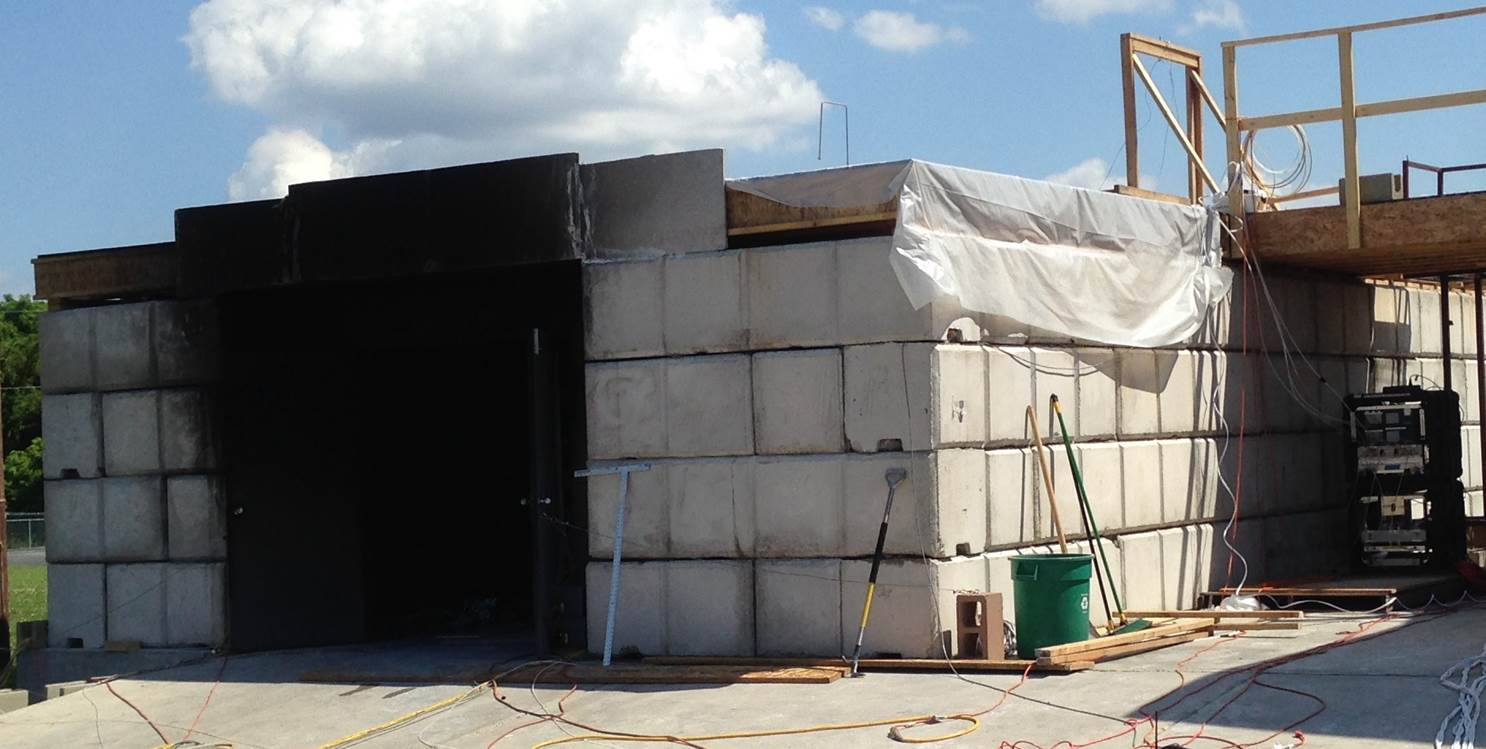
\includegraphics[width=5.25in]{../../Hose_Stream_Report/Figures/Pictures/east_structure}
	\\~\\
	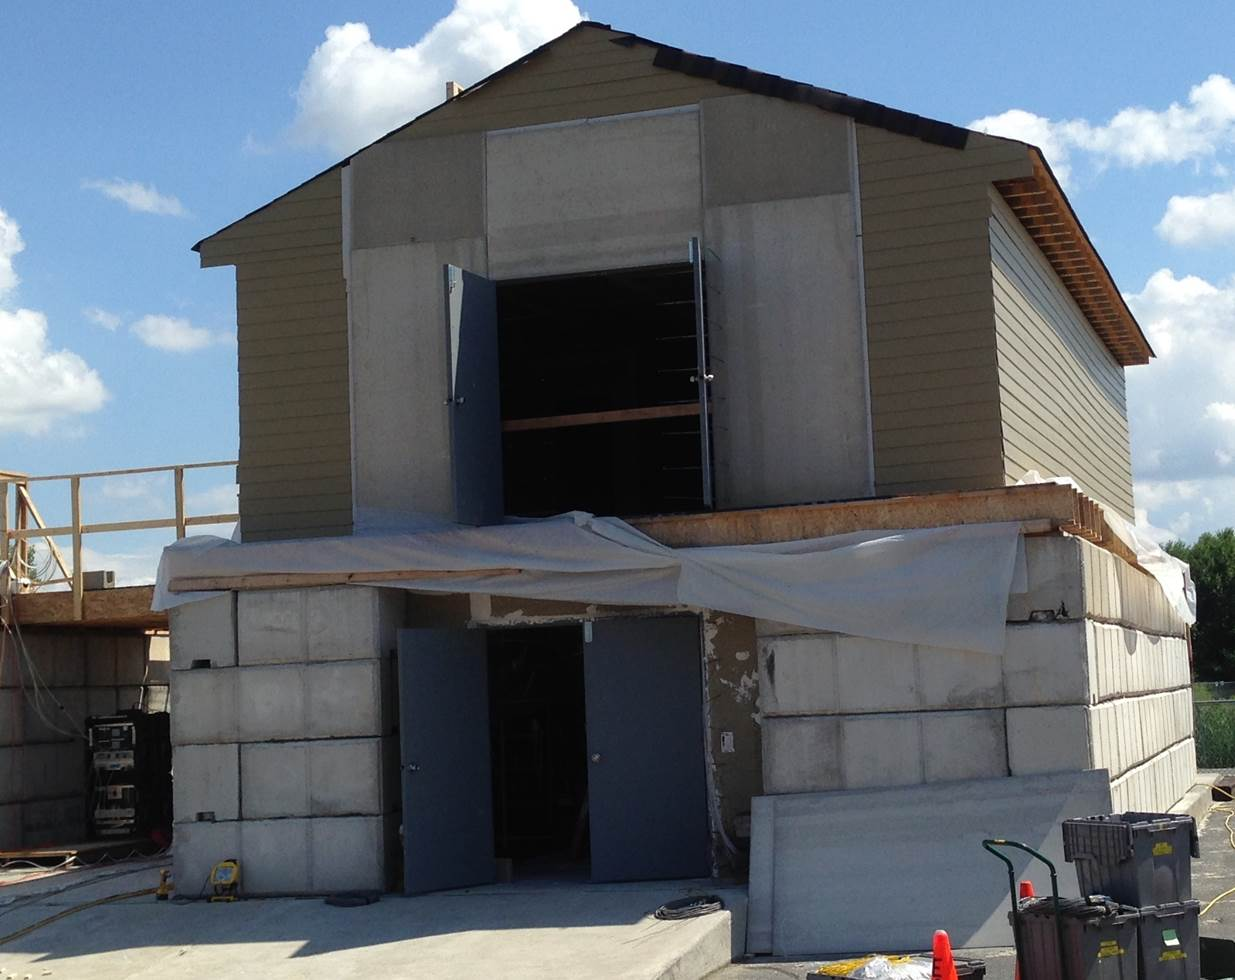
\includegraphics[width=5.25in]{../../Hose_Stream_Report/Figures/Pictures/west_structure}
	\caption[North side of the East and West Structures.]{North side of the East (top) and West (bottom) Test Structures.}
	\label{fig:struct_pics}
\end{figure}

The interior walls of the first floor of each structure were framed with steel studs set to 0.40~m (16~in) centers and track and \textit{were lined with 13~mm (0.5~in) thick cement board. The walls were composed of 16~mm (5/8~in) Type X gypsum board. Additionally, the ceiling was composed of two layers of 13~mm (0.5~in) thick cement board.}
\FloatBarrier

The first floor ceiling support of each structure was composed of wood truss joist I-beams (TJIs) with a 299~mm (11.75~in) depth. Each TJI was composed of laminated veneer lumber flanges with a cross section of 29~mm (1.13~in) x 44~mm (1.75~in) and an 11~mm (0.43~in) thick oriented strand board web as shown in Fig.~\ref{fig:TJI}. Tongue and grove, 18.3~mm (0.72~in) thick, oriented strand board was screwed to the top of the TJIs.

\begin{figure}[!ht]
	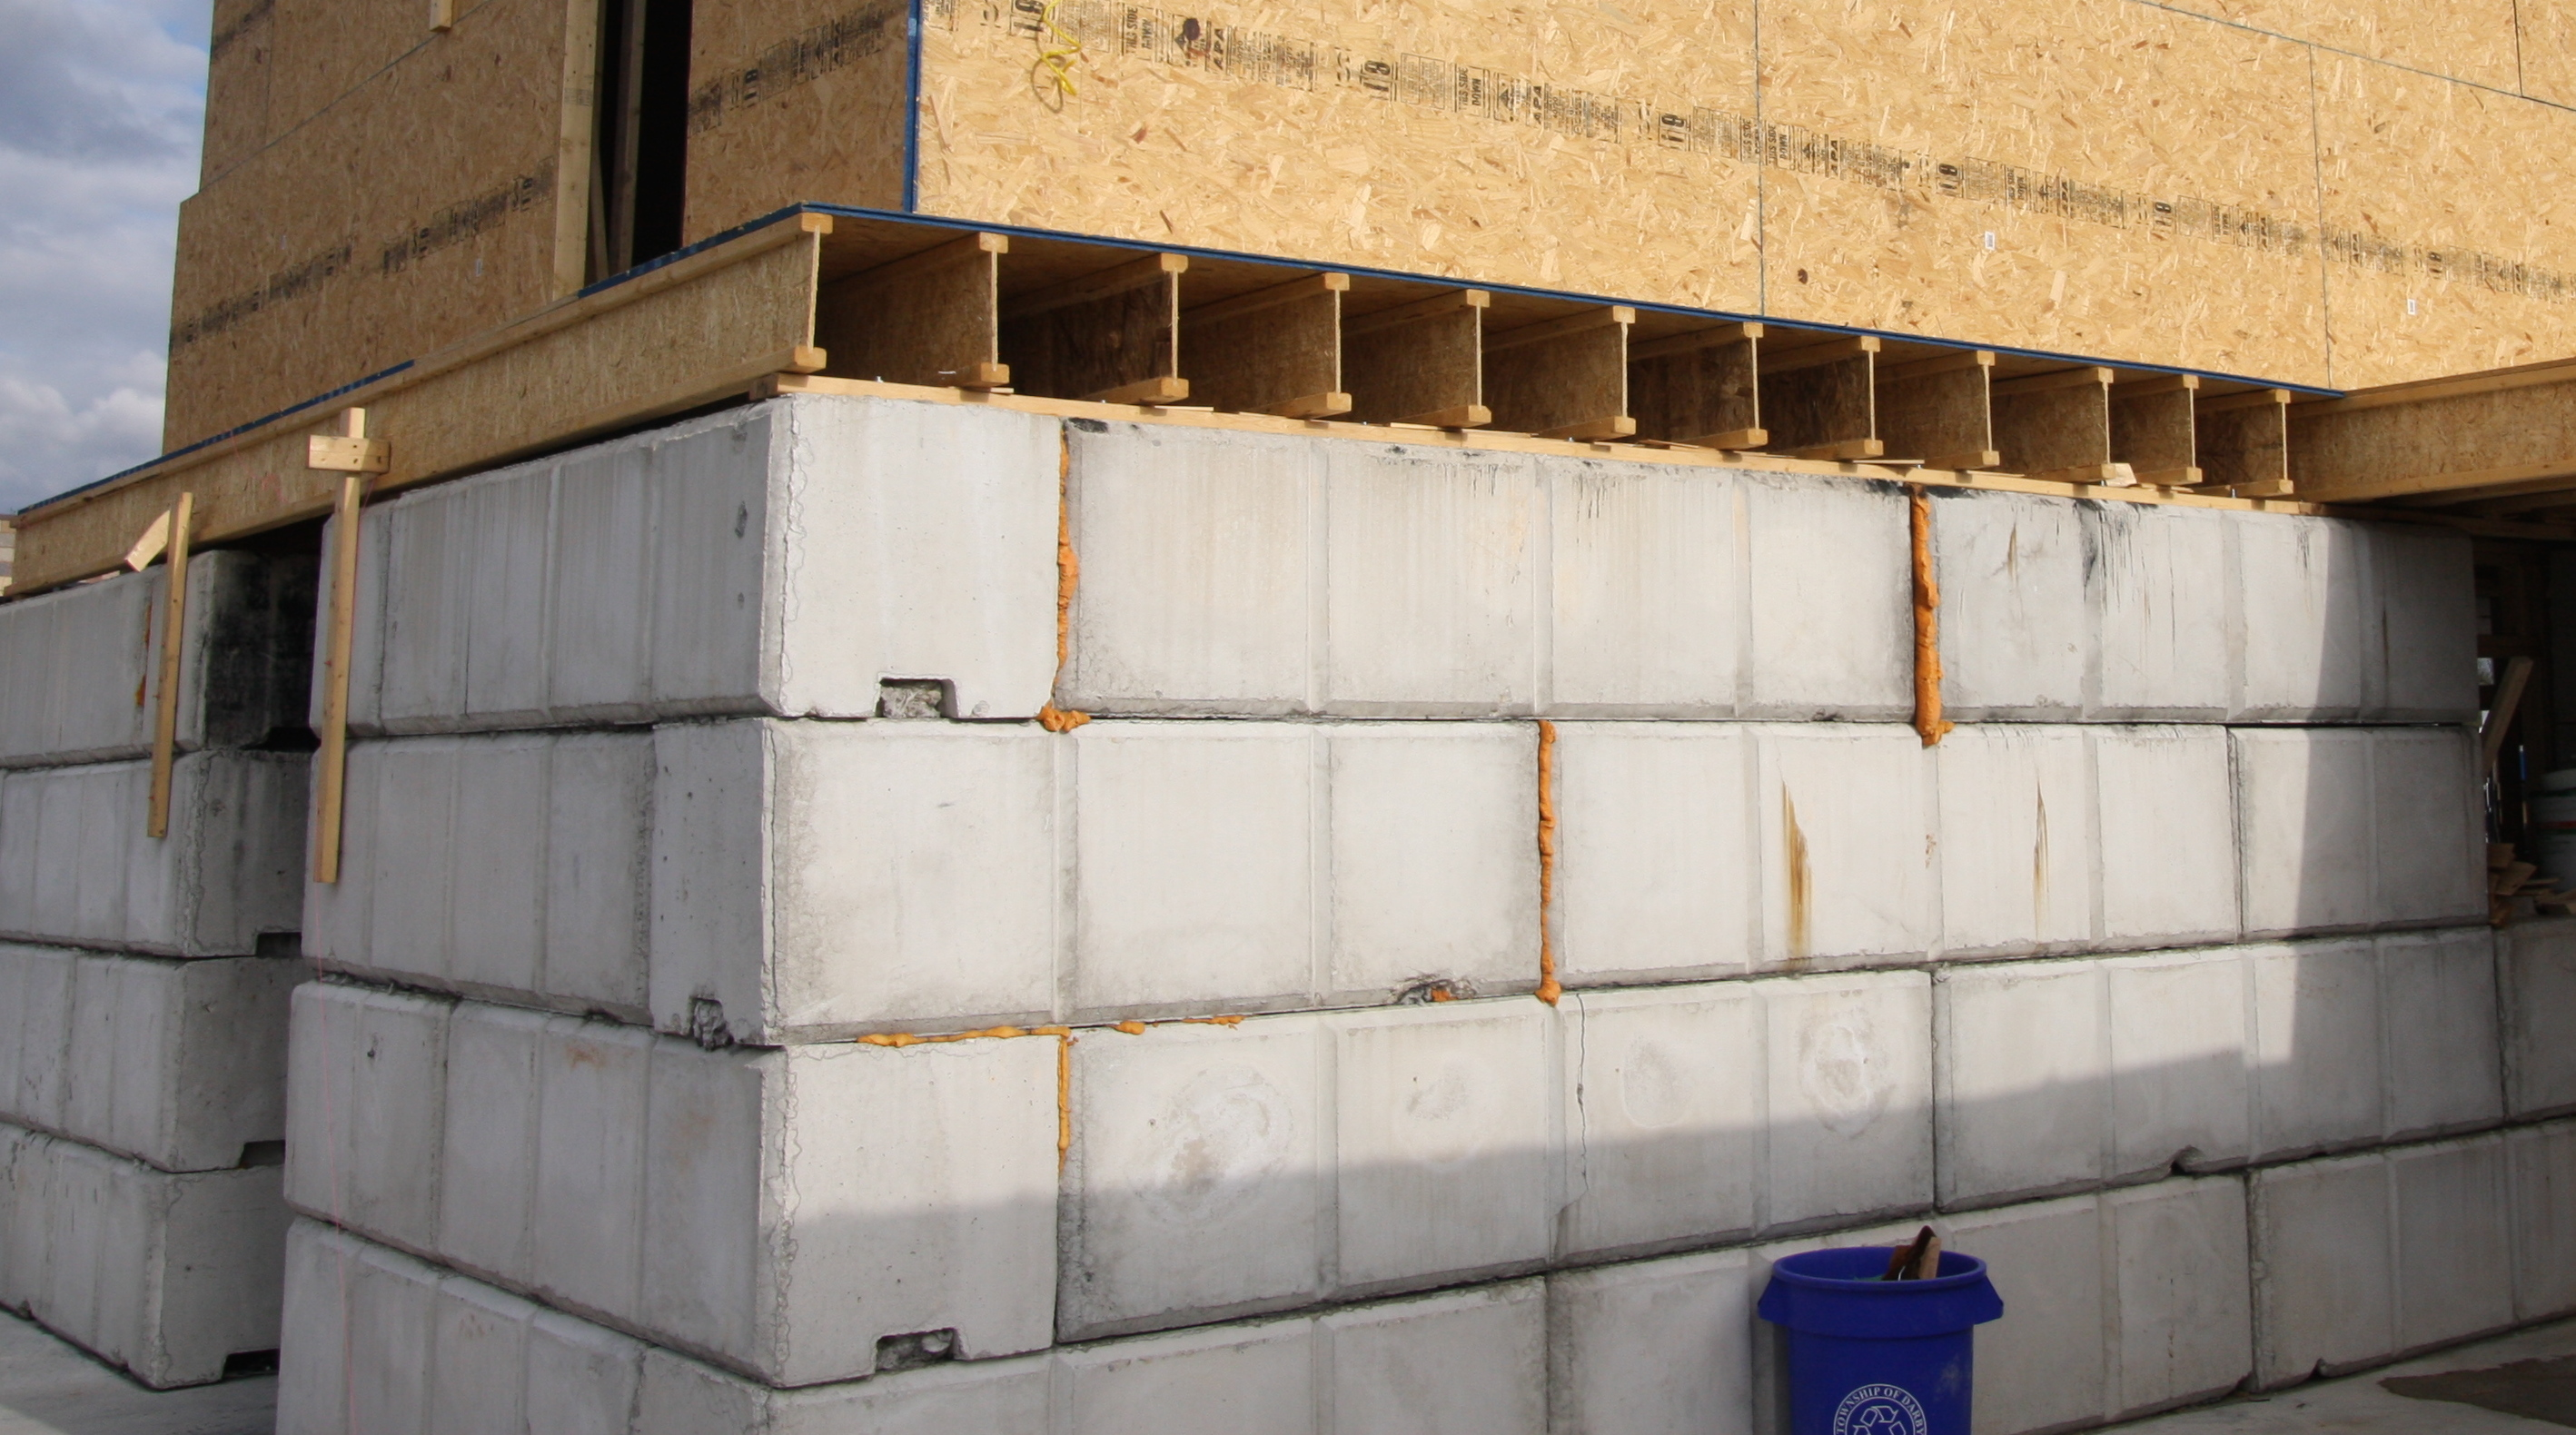
\includegraphics[width=6in]{../../Hose_Stream_Report/Figures/Pictures/TJI_support}
	\caption[TJI-constructed ceiling support of the West Structure.]{First floor ceiling support of the West Structure composed of wood truss joist I-beams. View is of the southeast corner of the structure.}
	\label{fig:TJI}
\end{figure}
\FloatBarrier

The second floor of the West Structure was built on the wood ceiling support described above and was connected to the first floor by a stairwell. The second story walls were wood framed with 51~mm (2~in) by 102~mm (4~in) studs set to 0.40~m (16~in) centers. The interior walls were protected by 16~mm (5/8~in) fire rated gypsum board, 16~mm (5/8~in) durarock board, and a second layer of 16~mm (5/8~in) fire rated gypsum board. The exterior walls were protected with 11~mm (7/16~in) oriented strand board and 8~mm (5/16~in) fiber cement lap siding.

% Add info about roof vent in single story
\subsection{Layout}
\label{sec:layout}
Dimensioned floor plans of the East and West Structures are presented in Figures~\ref{fig:east_dimensioned_plan}~and~\ref{fig:west_dimensioned_plan}, respectively.

\begin{figure}[!ht]
	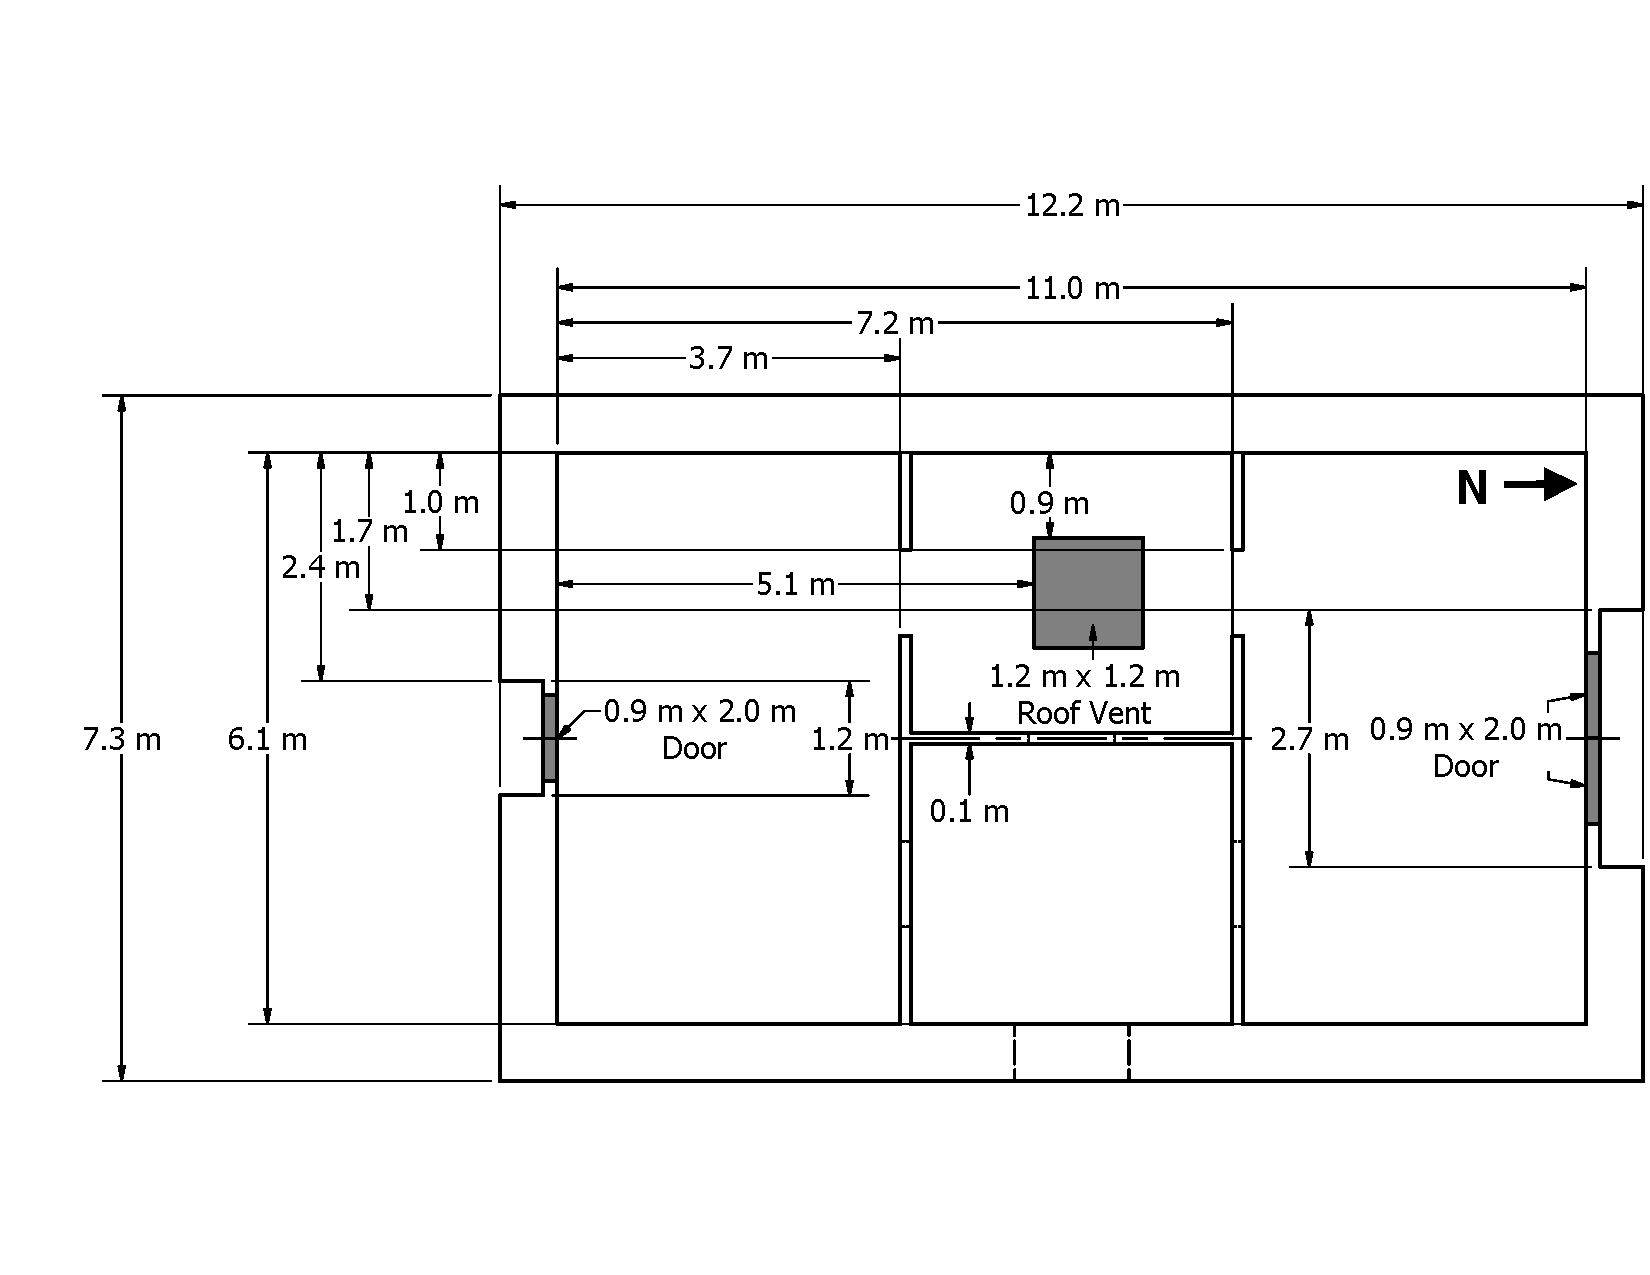
\includegraphics[width=\columnwidth]{../Figures/Floor_Plans/East_Structure_Dimensioned_Full}
	\caption[Dimensioned floor plan of the East Structure.]{East Structure floor layout.}
	\label{fig:east_dimensioned_plan}
\end{figure}
% make new floor plan with ceiling vent included

\begin{figure}[!ht]
	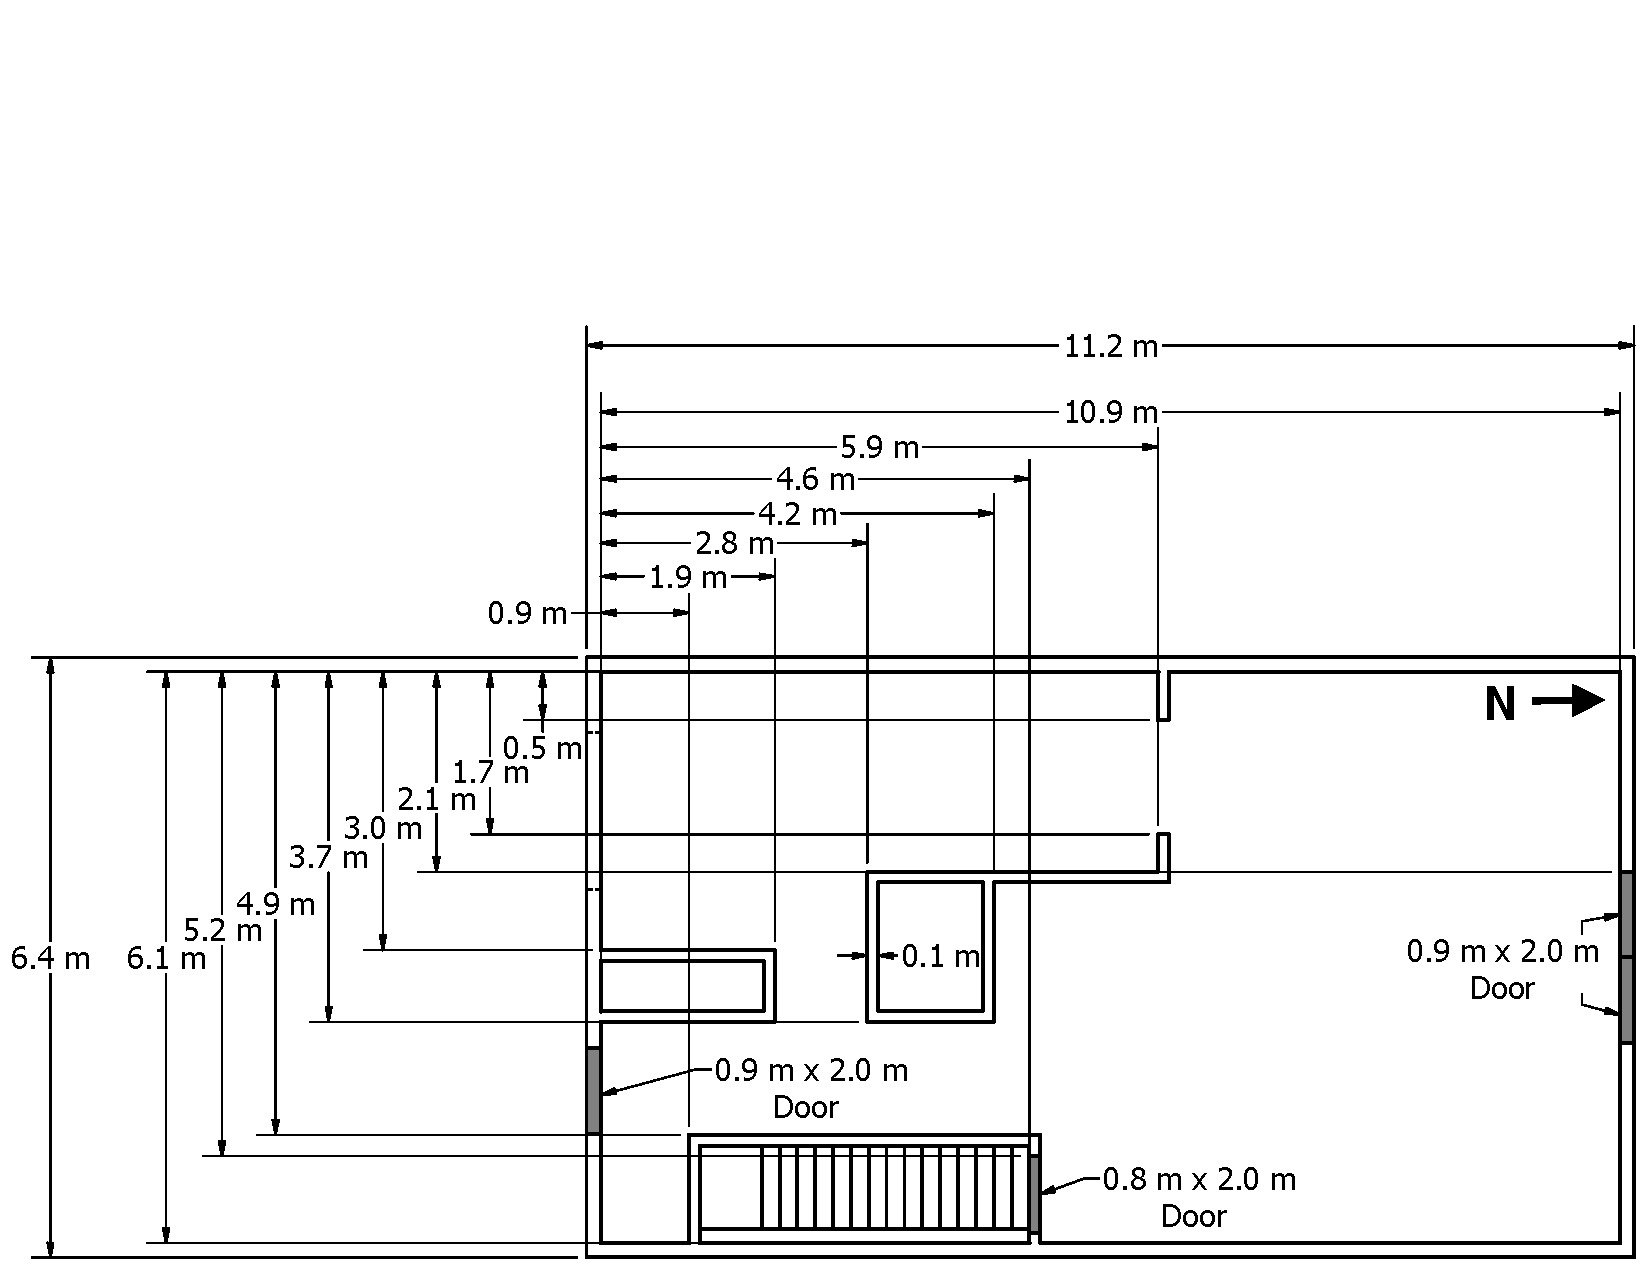
\includegraphics[width=\columnwidth]{..//Figures/Floor_Plans/West_Structure_2nd_Floor_Dimensioned_Full}
	\\~\\
	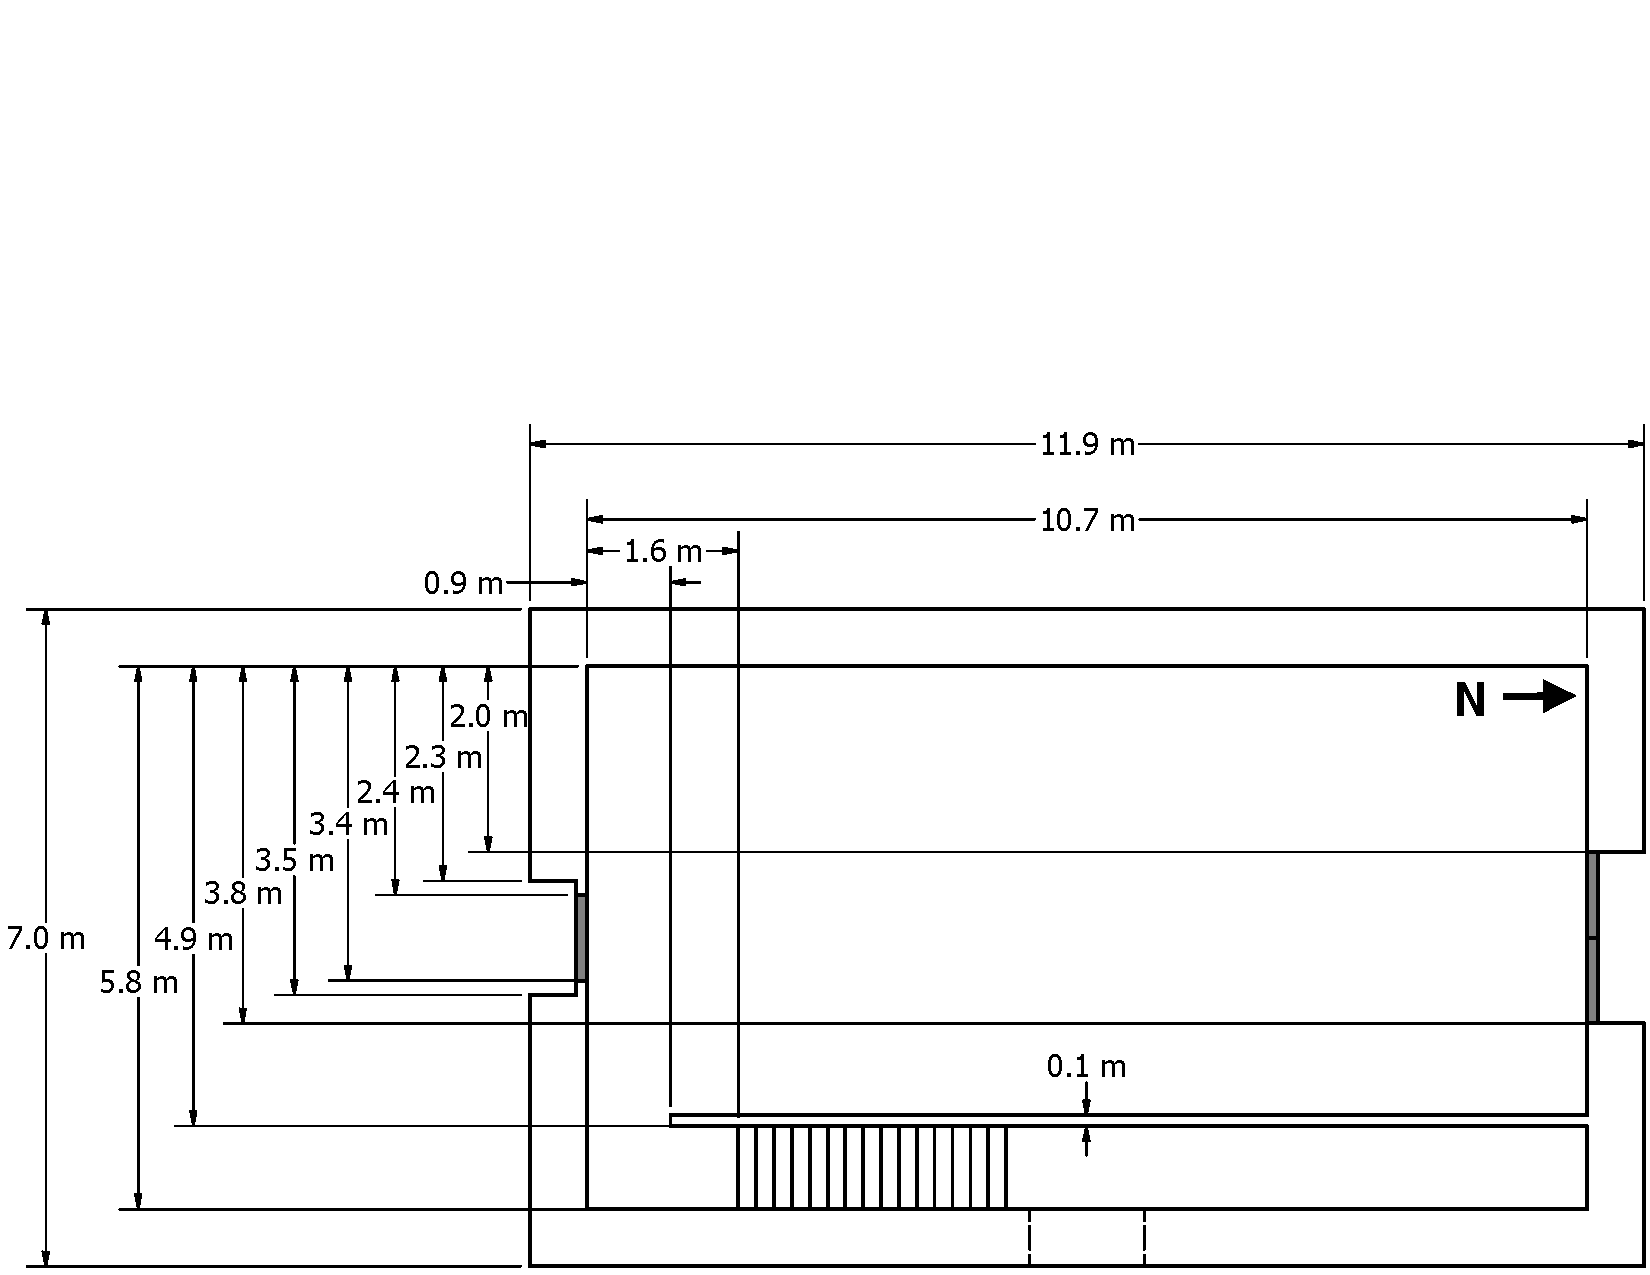
\includegraphics[width=\columnwidth]{../Figures/Floor_Plans/West_Structure_1st_Floor_Dimensioned_Full}
	\caption[Dimensioned floor plans of the West Structure.]{Dimensioned floor plan of the second floor (top) and first floor (bottom) of the West Structure.}
	\label{fig:west_dimensioned_plan}
\end{figure}

The interior dimensions of each structure were approximately 6.1~m (20~ft) wide, 11~m (36~ft) long and 2.4~m (8~ft) high. The stairs connecting the two floors of the West Structure started 1.6~m (5.25~ft) off the south wall with a width of 1.2~m (4~ft) off the east wall.

The exterior doorways of each structure and the stairwell doorway on the second level of the West Structure all contained doors that were opened or closed at certain instances to change the ventilation patterns of the structure. All other doorways in the structures did not contain a door, so to close the doorway, a sheet of gypsum board was used to cover the opening and the doorway remained closed for the duration of the test procedure.
\FloatBarrier

\section{Instrumentation}
\label{sec:Instrumentation}
The structures were instrumented for temperature, gas velocity, heat flux, and gas concentration measurements. Gas temperatures in the burn rooms were measured with bare-bead, Chromel-Alumel (type K) thermocouples. Additional single thermocouples were installed in conjunction with the bi-directional probes for gas velocity measurements. The single thermocouples were bare-bead, Chromel-Alumel (type K) thermocouples with a 1.0~mm (0.04~in) nominal diameter. The thermocouple wire was protected with an 3.2~mm (0.125~in) diameter inconel sheath. Schmidt-Boelter gauges were used to measure both total heat flux and radiant heat flux (radiometer). A radiometer is a total heat flux gauge with a zirconium plate to prevent contributions from convective heat transfer. Calibrated pumps pulled gas samples through a sample conditioning system to eliminate moisture in the sample. Then, the dry gas sample was piped to a series of gas analyzers and the concentrations of oxygen, carbon monoxide, and carbon dioxide were measured. A legend is presented in Fig.~\ref{fig:Instrumentation_Legend} to clarify the instrumentation schematics discussed in the follow sections.

\begin{figure}[!ht]
	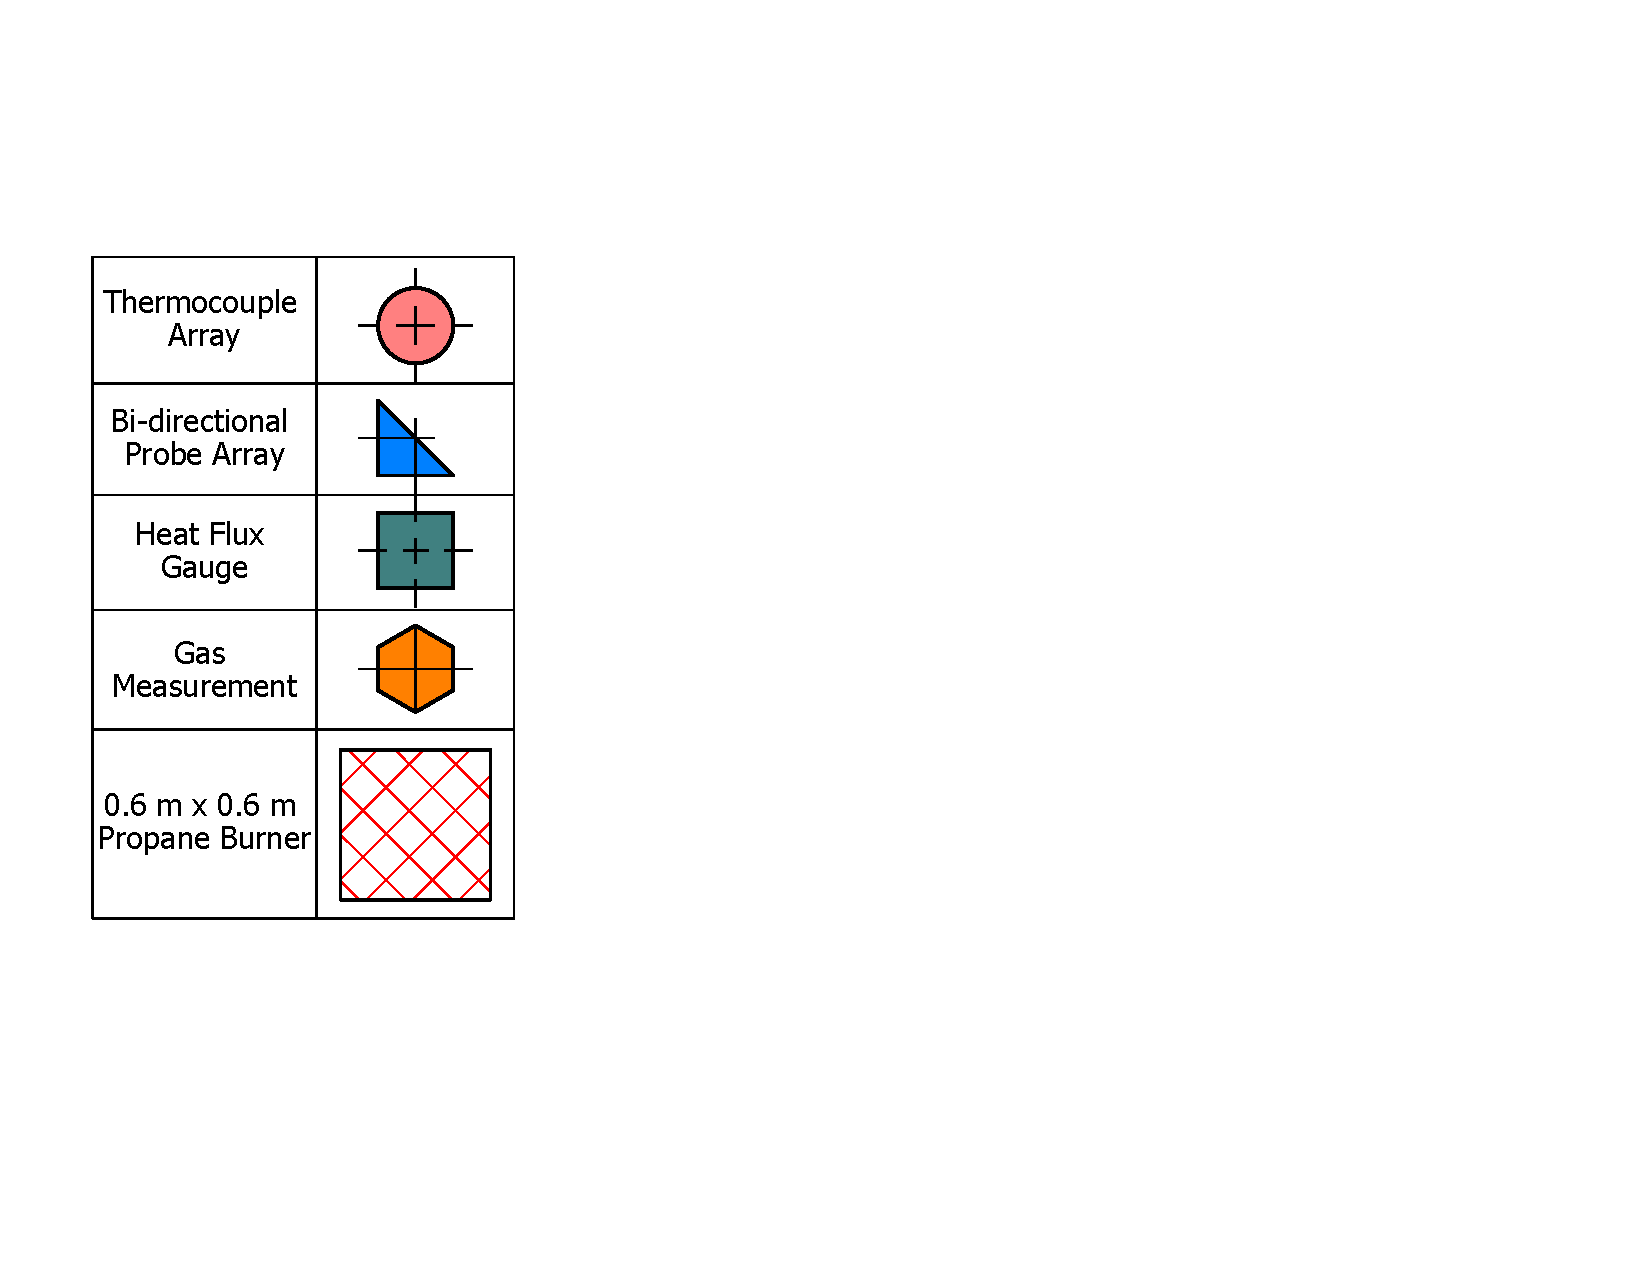
\includegraphics[width=0.25\columnwidth]{../Figures/Floor_Plans/Instrumentation_Legend}
	\caption{Instrumentation Legend.}
	\label{fig:Instrumentation_Legend}
\end{figure}

Three propane burners, each with a square opening of side length 0.6~m (2~ft) 0.14~m (5.5~in) above the floor, were positioned 0.6~m (2~ft) from the south and west walls on the first floor of each structure and used as the fuel source in each experiment. Propane flowed at a known volumetric flow rate during the experiments.
\FloatBarrier

\subsubsection*{East Structure}
The East Structure was instrumented with 5 bare-bead thermocouple arrays, 4 bi-directional probe plus solid thermocouple arrays, 5 total heat flux plus radiometer sensor pairs, and 2 gas sample inlet pipes at the locations shown in Fig.~\ref{fig:east_instrumentation}.

\begin{figure}[!ht]
	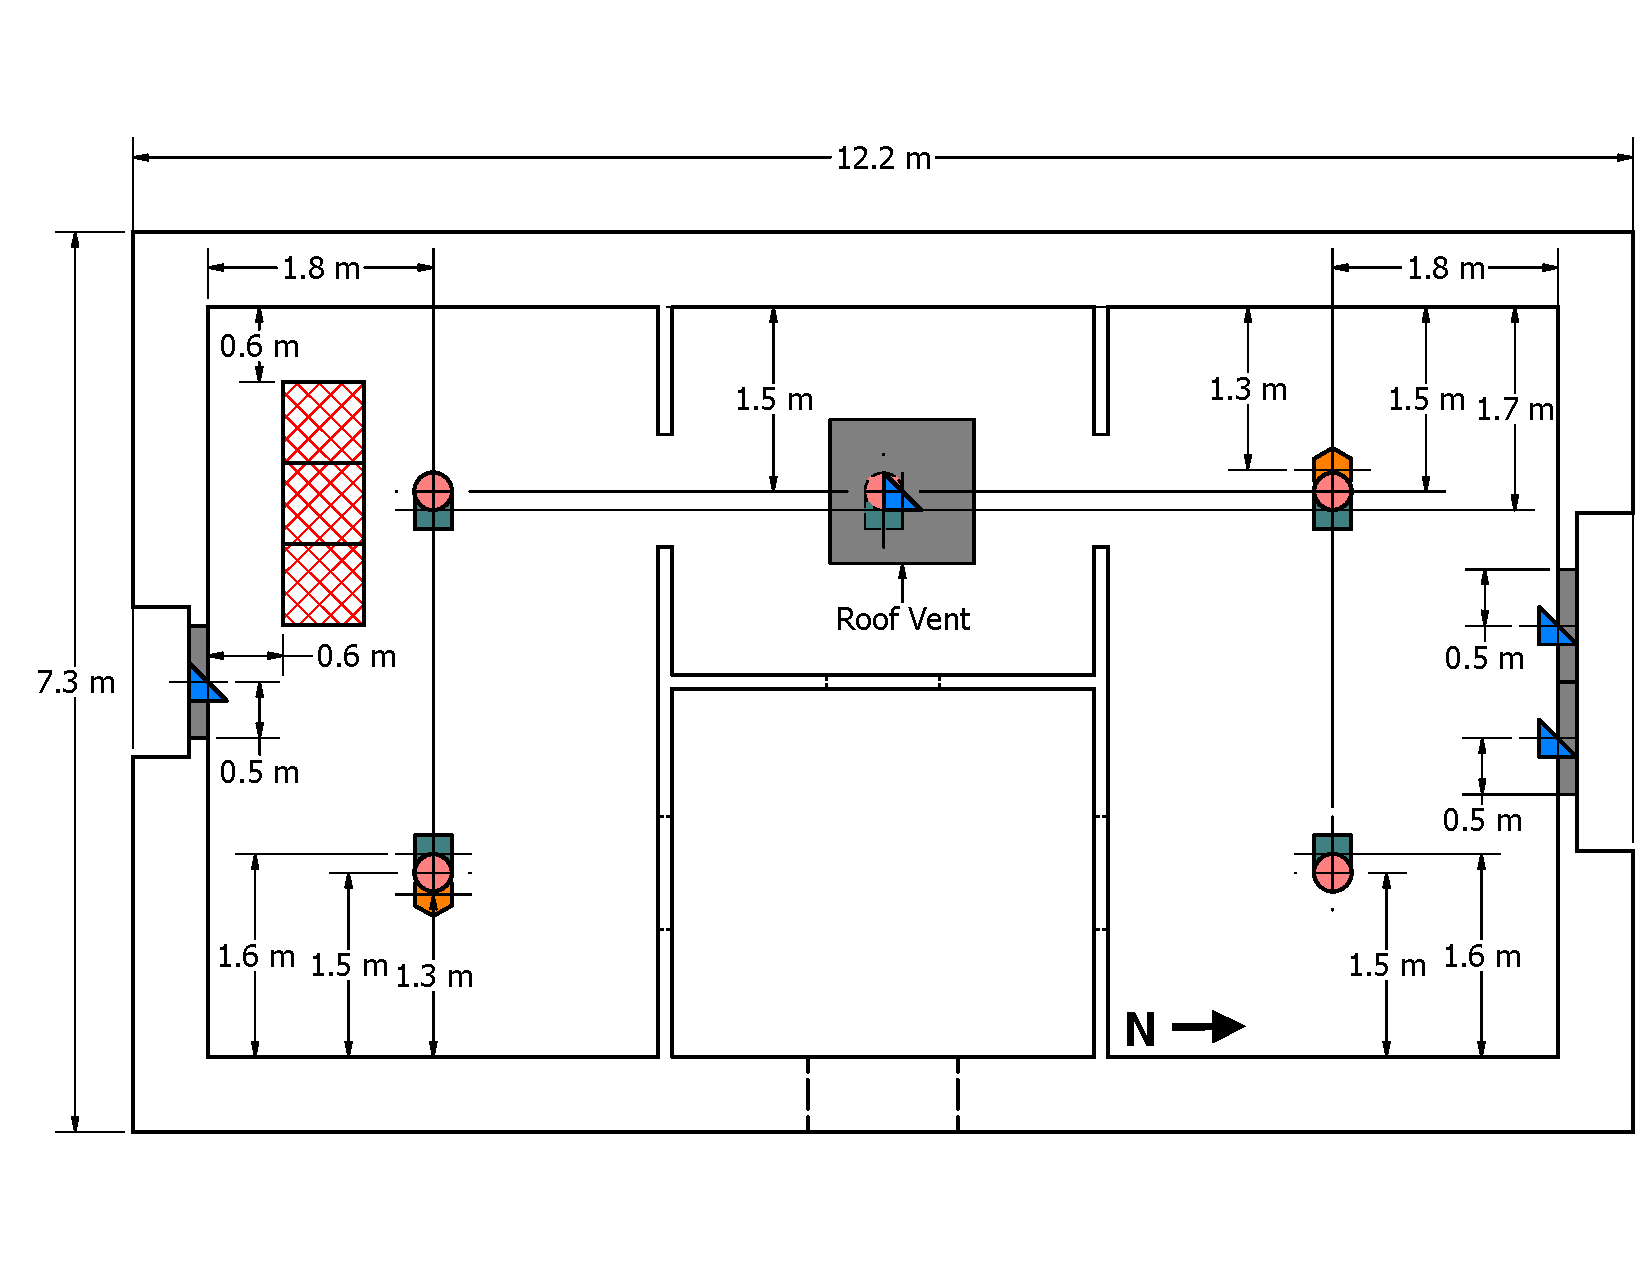
\includegraphics[width=\columnwidth]{../Figures/Floor_Plans/East_Structure_Dimensioned_Instrumentation}
	\caption{Location of instrumentation in the East Structure.}
	\label{fig:east_instrumentation}
\end{figure}

Each bare-bead thermocouple array was composed of 8 thermocouples. The top sensor was 0.03~m (1~in) below the ceiling and the remaining thermocouples were space 0.3~m (1~ft) apart with the bottom thermocouple being 2.13~m (7~ft) below the ceiling. The three bi-directional probe and solid thermocouple arrays located at the exterior doorways of the structure contained 8 probes centered in the doorway with the first probe 0.08~m (0.25~ft) below the soffit and the remaining probes at 0.34~m (1.1~ft), 0.61~m (2~ft), 0.88~m (2.9~ft), 1.15~m (3.7~ft), 1.42~m (4.7~ft), 1.68~m (5.5~ft), and 1.95~m (6.4~ft) below the soffit. The fourth bi-directional probe and solid thermocouple array was located at the roof vent and contained three probes \textit{centered between the east and west sides of the vent and spaced ?? apart between the north and south sides.} The total heat flux guage/radiometer pairs were set to be 0.15~m (0.5~ft) off the ground and aimed to view the ceiling. Gas concentrations were pulled through \textit{3.2~mm (0.125~in) diameter stainless steel tubing located 1.22~m (4~ft) above the floor.}
\FloatBarrier

\subsubsection*{West Structure}
The first floor of the West Structure was instrumented with 3 bare-bead thermocouple arrays, 3 bi-directional probe plus solid thermocouple arrays, and 1 gas sample inlet pipe, and the second floor was equipped with 3 bare-bead thermocouple arrays, 4 bi-directional probe plus solid thermocouple arrays, and 1 gas sample inlet pipe. The locations of the instrumentation in the West Structure is shown in Fig.~\ref{fig:west_instrumentation}.

\begin{figure}[!ht]
	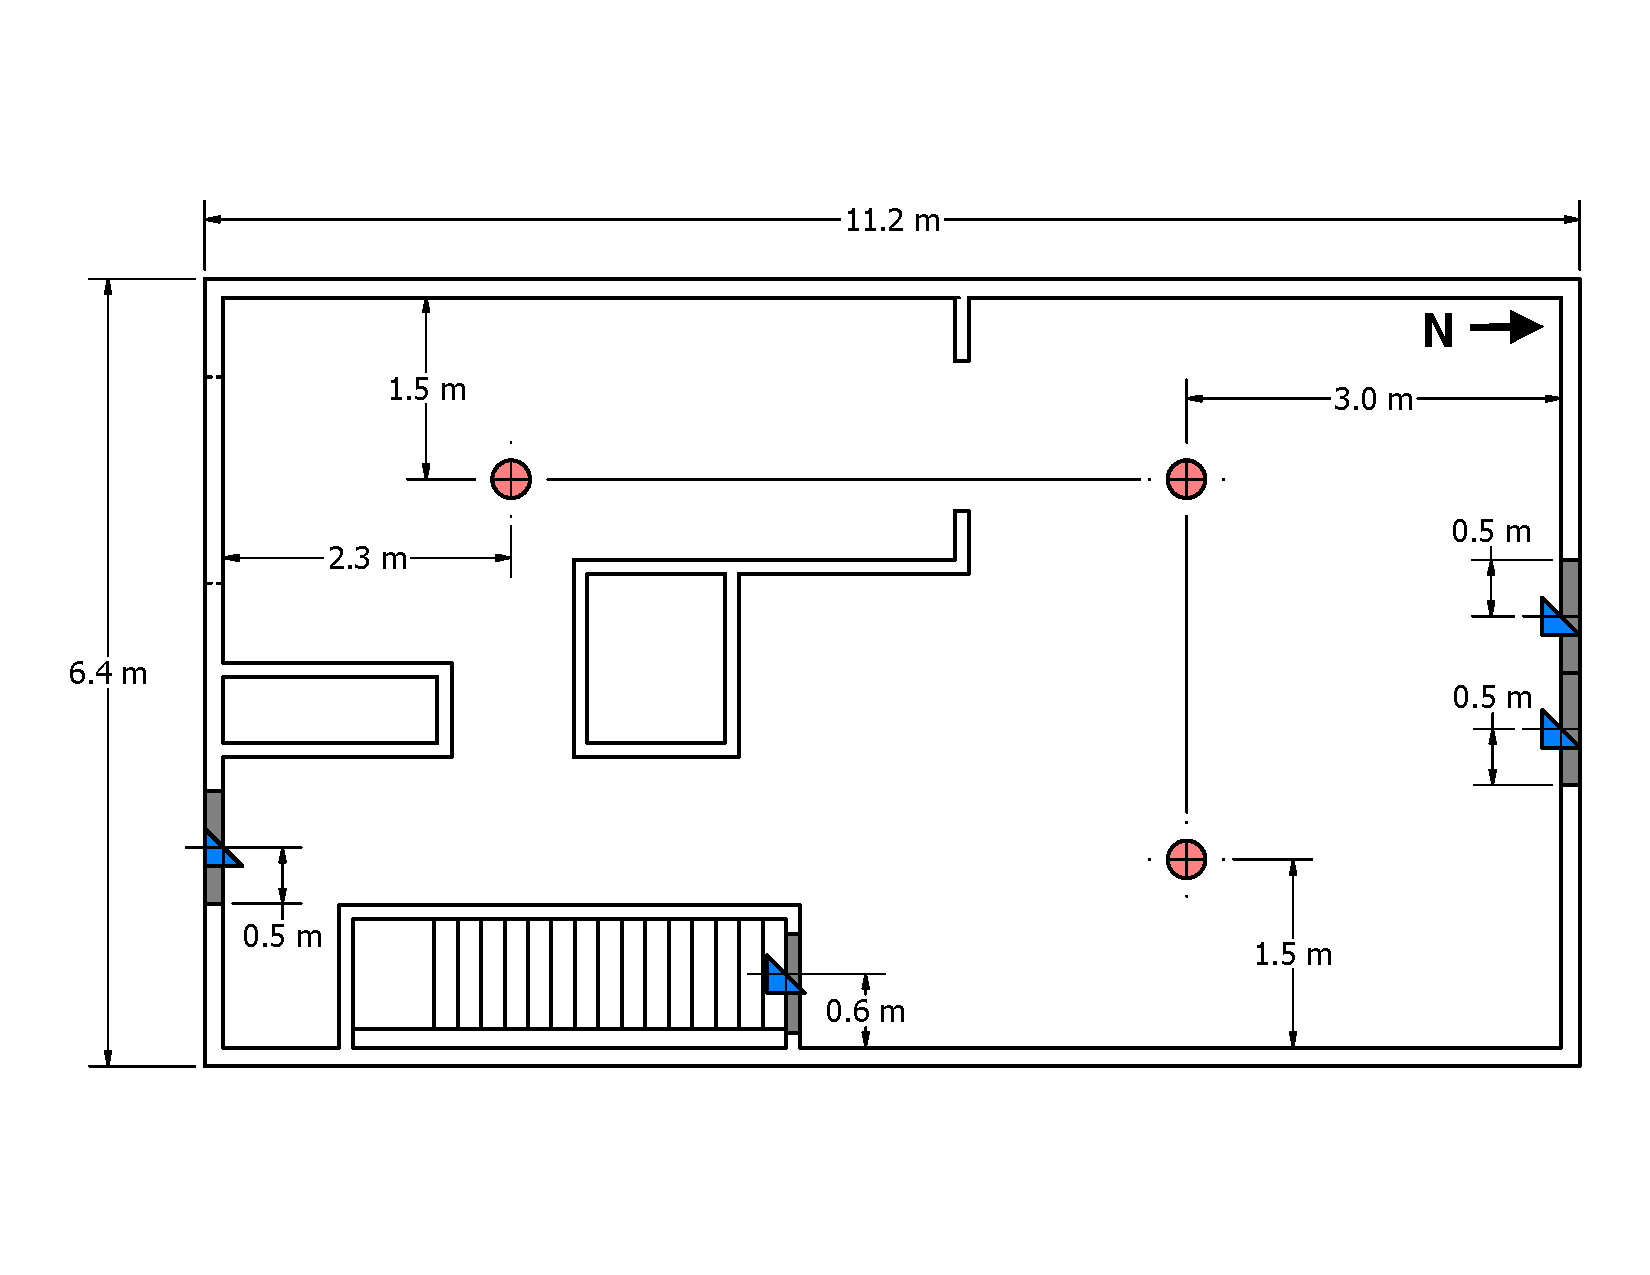
\includegraphics[width=\columnwidth]{../Figures/Floor_Plans/West_Structure_2nd_Floor_Dimensioned_Instrumentation}
	\\~\\
	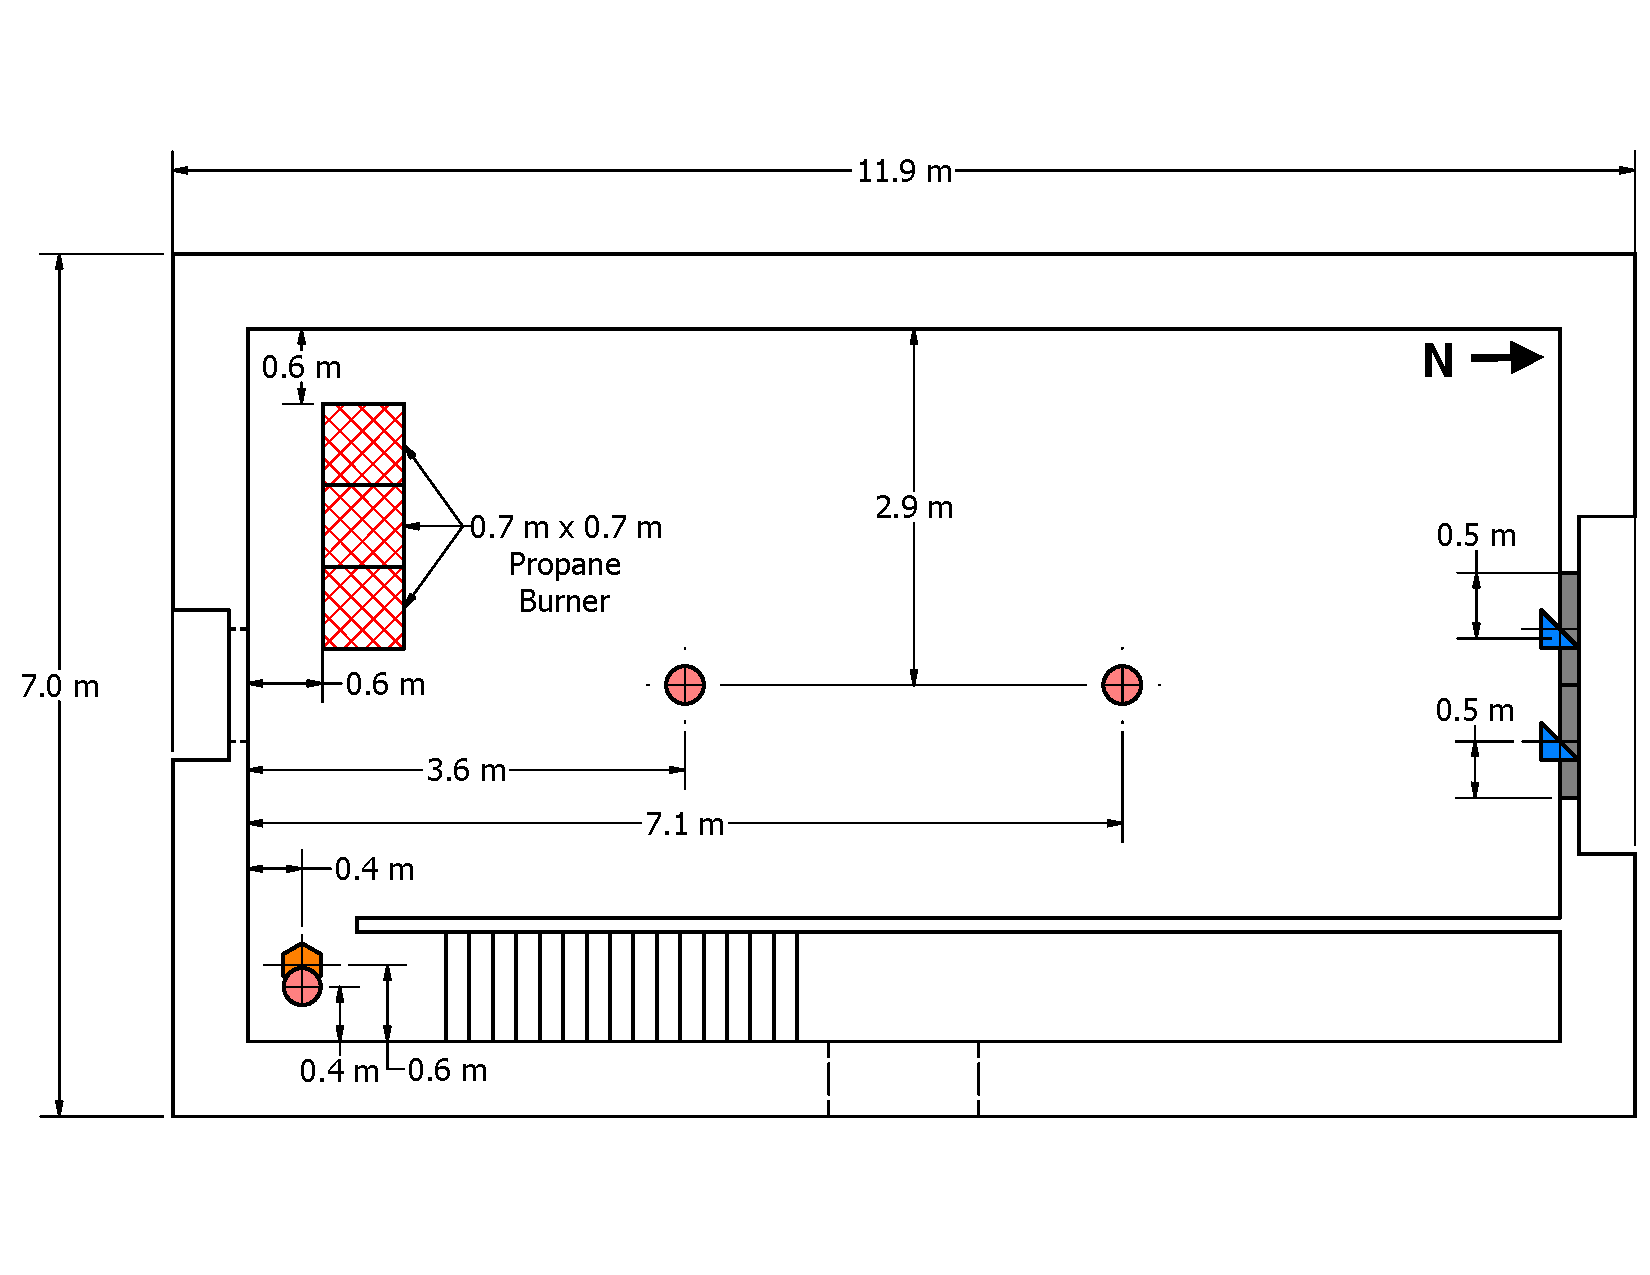
\includegraphics[width=\columnwidth]{../Figures/Floor_Plans/West_Structure_1st_Floor_Dimensioned_Instrumentation}
	\caption[Location of instrumentation in the West Structure.]{Location of instrumentation in the second floor (top) and first floor (bottom) of the West Structure.}
	\label{fig:west_instrumentation}
\end{figure}

The thermocouples in the bare-bead thermocouple arrays were spaced in the same manner as the arrays in the East Structure. The bi-directional probe and thermocouple arrays contained 8 probes with spacing identical to the arrays at the exterior doors of the East Structure. 3.2~mm (0.125~in) stainless steel tubing was located 1.22~m (4~ft) above the floor and used to pull gas samples from the environment. 
\FloatBarrier

\subsection{Measurement Uncertainty}
\label{sec:Uncertainty}
There are different components of uncertainty in the reported length, mass, temperature, heat flux, gas concentration, differential pressure, and gas velocity measurements. Uncertainties are grouped into two categories according to the method used to estimate them. Type A uncertainties are those which are evaluated by statistical methods, and Type B are those which are evaluated by other means~\cite{Taylor&Kuyatt:1994}. Type B analysis of systematic uncertainties involves estimating the upper (+a) and lower (-a) limits for the quantity in question such that the probability that the value would be in the interval ($\pm$a) is essentially 100\%. After estimating uncertainties by either Type A or B analysis, the uncertainties are combined in quadrature to yield the combined standard uncertainty. Then the combined standard uncertainty is multiplied by a coverage factor of two, which results in the expanded uncertainty with a 95\% confidence interval (2$\sigma$). For some of these components, such as the zero and calibration elements, uncertainties are derived from referenced instrument specifications. For other components, referenced research results and past experience with the instruments provided input in the uncertainty determination.

Each length measurement was taken carefully. Length measurements such as the room dimensions, instrumentation array locations, and fire apparatus (e.g., nozzle, sprinkler, or fan) placement were made with a hand held laser measurement device which has an accuracy of $\pm$6.0~mm (0.25~in) over a range of 0.61~m (2.0~ft) to 15.3~m (50.0~ft)~\cite{StanleyTools}. However, conditions affecting the measurement, such as levelness of the device, yields an estimated uncertainty of $\pm$0.5\% for measurements in the 2.0~m (6.6~ft) to 10.0~m (32.8~ft) range. Steel measuring tapes with a resolution of $\pm$0.5~mm (0.02~in) were used to locate individual sensors within a measurement array and to measure and position the furniture. The steel measuring tapes were manufactured in compliance with NIST Manual 44, which specifies a tolerance of $\pm$1.6~mm (0.06~in) for 9.1~m (30~ft) tapes and $\pm$6.4~mm (0.25~in) for 30.5~m (100~ft) tapes~\cite{Butcher:2012}. Some issues, such as ``soft'' edges on the upholstered furniture, result in an estimated total expanded uncertainty of $\pm$1.0\%.

The standard uncertainty in temperature of the thermocouple wire itself is $\pm$2.2$^{\circ}$C at $277^{\circ}$C and increases to $\pm$9.5$^{\circ}$C at $871^{\circ}$C as determined by the wire manufacturer~\cite{Omega:2004}. The variation of the temperature in the environment surrounding the thermocouple is known to be much greater than that of the wire uncertainty~\cite{Blevins:1999,Pitts:2003}. Small diameter thermocouples were used to limit the impact of radiative heating and cooling. The estimated total expanded uncertainty for temperature in these experiments is $\pm$15\%.

In this study, total heat flux measurements were made with water-cooled Schimidt-Bolter gauges. The manufacturer reports a $\pm$3\% calibration expanded uncertainty for these devices~\cite{Medtherm:2003}. Results from an international study on total heat flux gauge calibration and response demonstrated that the uncertainty of a Schmidt-Boelter gauge is typically $\pm$8\%~\cite{Pitts:2006}.

The gas measurement instruments and sampling system used in this series of experiments have demonstrated an expanded (k = 2) relative uncertainty of $\pm$1\% when compared with span gas volume fractions~\cite{Bundy:2007}. Given the non-uniformities and movement of the fire gas environment and the limited set of sampling points in these experiments, an estimated uncertainty of $\pm$12\% is associated with gas concentration measurements~\cite{Lock:1}.

Differential pressure reading uncertainty components were derived from pressure transducer instrument specifications and previous experience with pressure transducers. The transducers were factory calibrated and the zero and span of each was checked in the laboratory prior to the experiments yielding an accuracy of $\pm$1\%~\cite{Setra:2002}. The total expanded uncertainty was estimated at 10\%.

Bi-directional probes and single thermocouples were used to measure the velocity. The bi-directional probes used similar pressure transducers as those used for the differential pressure measurements discussed above. A single bare-bead Chromel-Alumel (type K) thermocouple with a 1.0~mm (0.04~in) nominal diameter was co-located with each probe. The thermocouple wire was protected with an 3.2~mm (0.125~in) diameter inconel sheath. A gas velocity measurement study examining the doorway flow of pre-flashover compartment fires yielded expanded uncertainty measurements ranging from $\pm$0.14 to $\pm$0.22 for bi-directional probes similar to the ones described here~\cite{Bryant:FSJ2009}. The total expanded uncertainty for gas velocity in these experiments was estimated to be $\pm$18\%.

\textit{Gas meter flowrate/HRR error}

% ==========================
% = EXPERIMENTAL PROCEDURE =
% ==========================
\chapter{Experimental Procedure}
\label{chap:Experimental_Procedure}
A similar procedure was followed for all experiments described in this report. First, three propane burners were ignited in sequential order. Next, different doors and vents in the structure were opened and closed to change the ventilation pattern within the structure. Finally, the burners were turned off in sequential order and the fire was extinguished. 

\section{East Structure Tests}
Three different test series---Series 4, Series 5, and Series 6---were conducted in the east structure. Each series was composed of three experiments that used an identical procedure to change the ventilation in the structure. The experiments conducted during Series 4 followed a procedure in which each exterior door was opened to change the ventilation pattern. During the experiments in Series 5, each double door was opened and the roof vent was opened and closed. Both the roof vent and west double door were opened during each experiment in Series 6. Figs.~\ref{fig:east_test_4}--\ref{fig:east_test_6} include a schematic and additional details about the procedures used for the experiments during Series 4--6.

\begin{figure}[!ht]
\begin{minipage}[b]{0.8\columnwidth}
	\begin{flushleft}
	\small
	\begin{tabular}[b]{cc}
 	\toprule
 	\textbf{Number} & \textbf{Event Description} \\
 	\midrule
 	1-3  & Burners ignited \\
 	4	 & West double door opened \\
 	5 	 & East double door opened \\
 	6	 & South side door opened \\
 	7-9  & Burners extinguished \\
	\bottomrule
	\end{tabular}
	\end{flushleft}
\end{minipage}
\begin{minipage}[b]{0.9\columnwidth}
	\vspace{15pt}
	\centering
	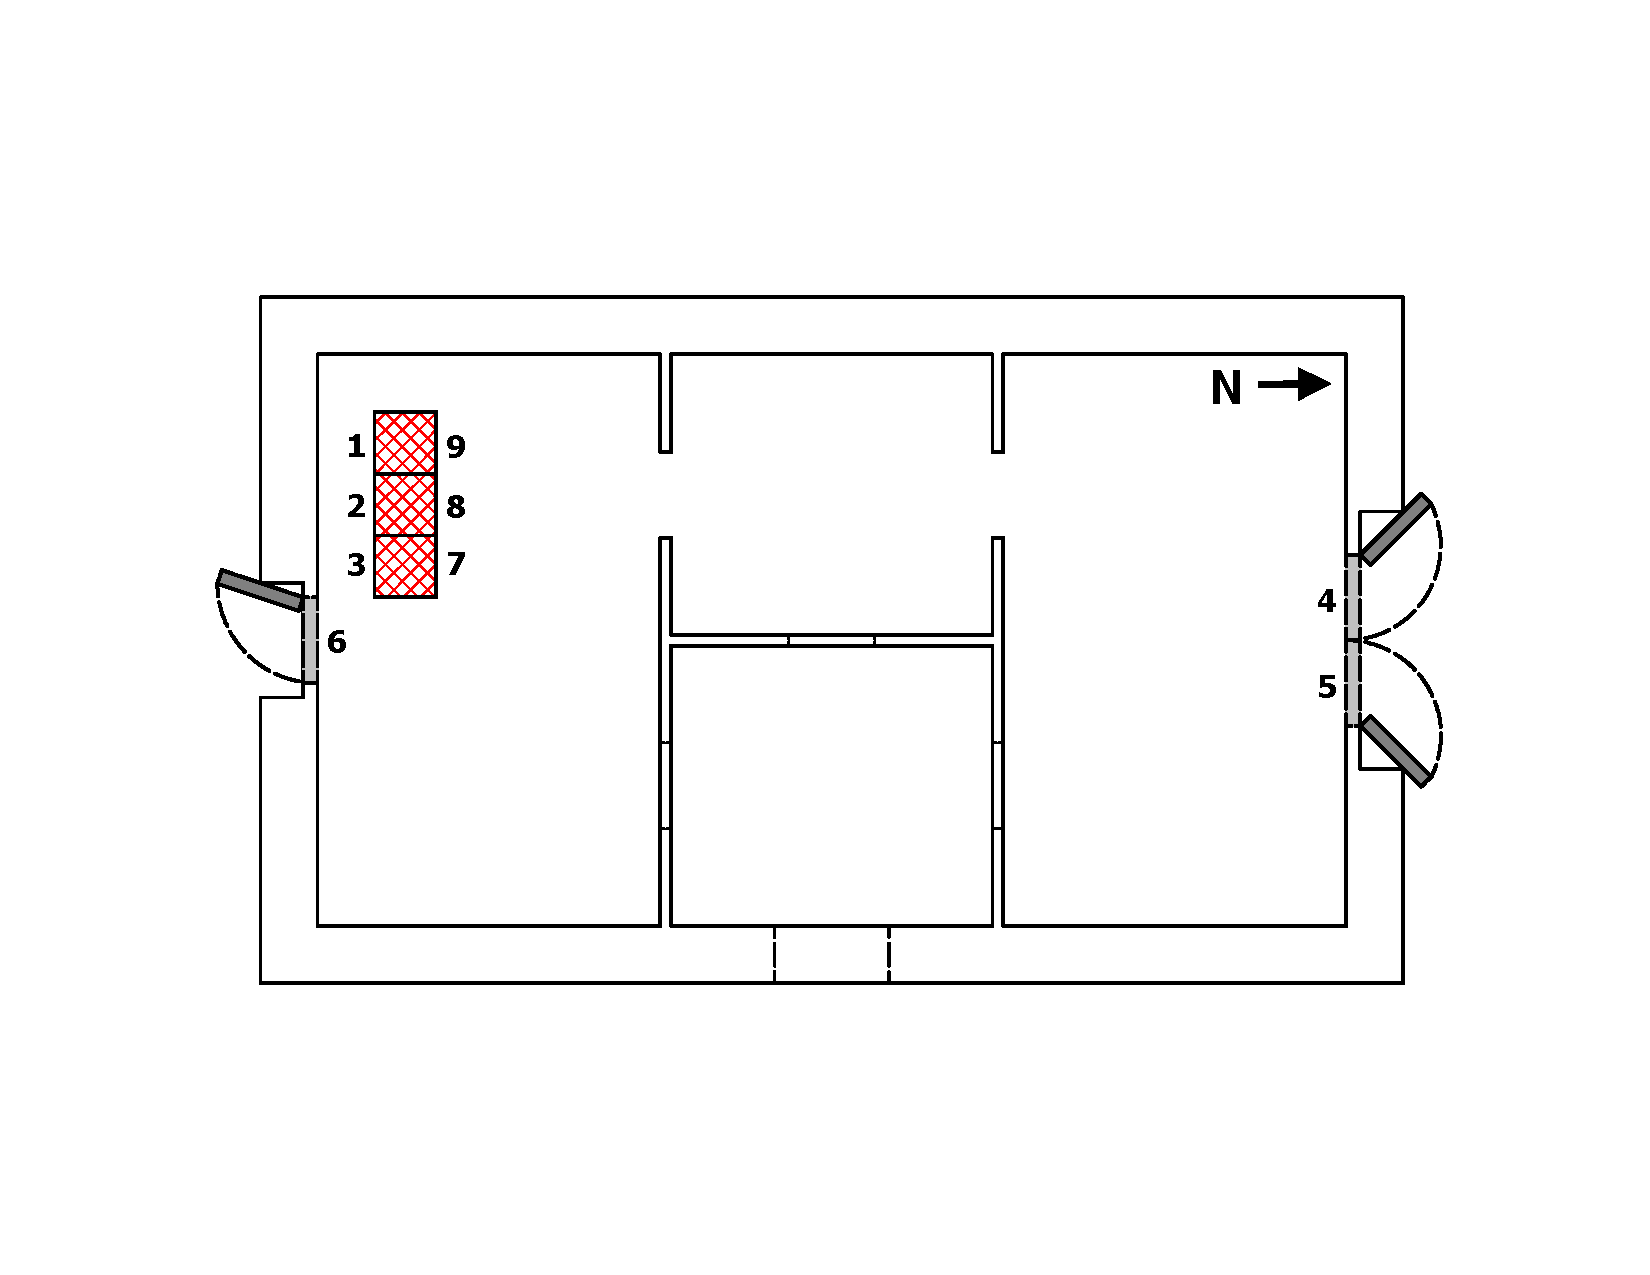
\includegraphics[width=\columnwidth]{../Figures/Floor_Plans/East_Structure_Test_4}
\end{minipage}
\caption{Test Series 4 layout and sequence of events.}
\label{fig:east_test_4}
\end{figure}

\begin{figure}[!ht]
\begin{minipage}[b]{0.8\columnwidth}
	\begin{flushleft}
	\small
	\begin{tabular}[b]{cc}
 	\toprule
 	\textbf{Number} & \textbf{Event Description} \\
 	\midrule
 	1-3  & Burners ignited \\
 	4	 & Roof vent opened \\
 	5 	 & West double door opened \\
 	6 	 & East double door opened \\	
 	7	 & Roof vent closed \\
 	8-10  & Burners extinguished \\
	\bottomrule
	\end{tabular}
	\end{flushleft}
\end{minipage}
\begin{minipage}[b]{0.9\columnwidth}
	\vspace{15pt}
	\centering
	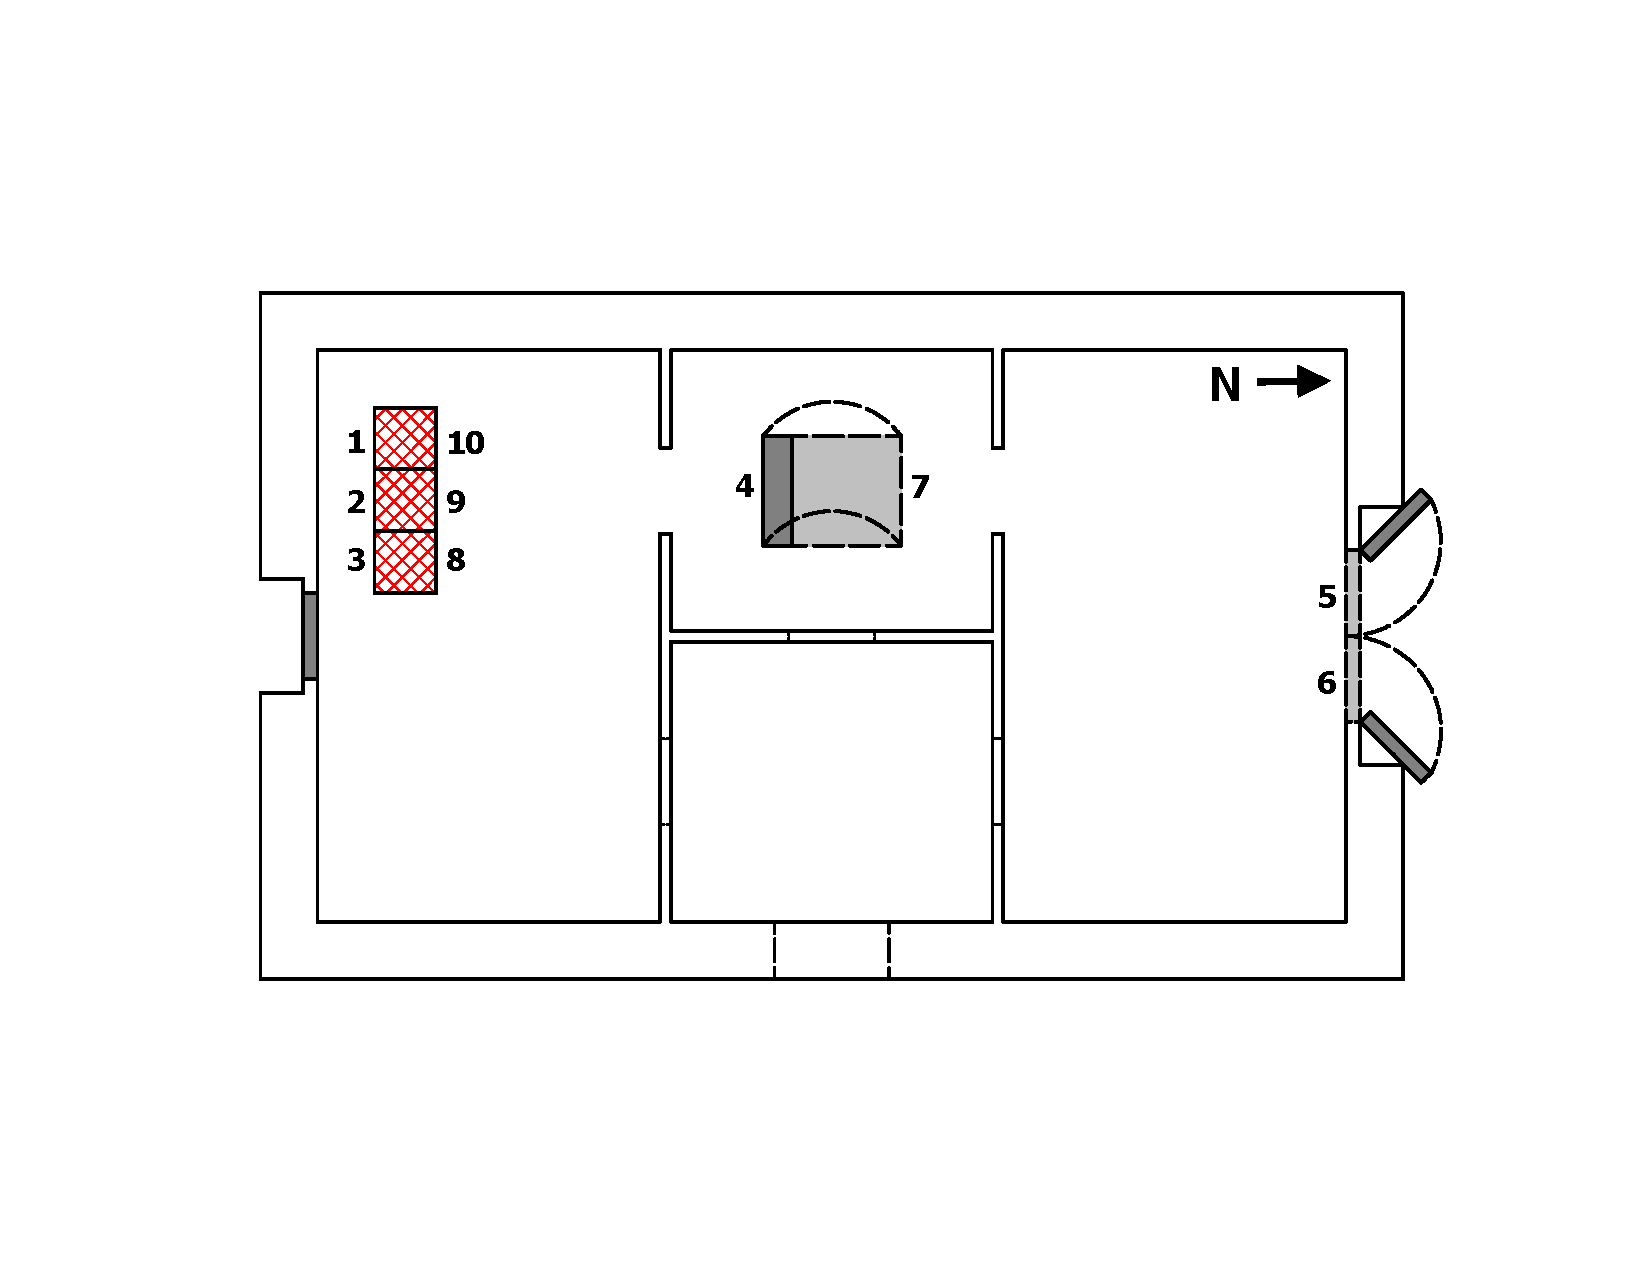
\includegraphics[width=\columnwidth]{../Figures/Floor_Plans/East_Structure_Test_5}
\end{minipage}
\caption{Test Series 5 layout and sequence of events.}
\label{fig:east_test_5}
\end{figure}

\begin{figure}[!ht]
\begin{minipage}[b]{0.8\columnwidth}
	\begin{flushleft}
	\small
	\begin{tabular}[b]{cc}
 	\toprule
 	\textbf{Number} & \textbf{Event Description} \\
 	\midrule
 	1-3  & Burners ignited \\
 	4	 & Roof vent opened \\
 	5 	 & West double door opened \\
 	6-8  & Burners extinguished \\
	\bottomrule
	\end{tabular}
	\end{flushleft}
\end{minipage}
\begin{minipage}[b]{0.9\columnwidth}
	\vspace{15pt}
	\centering
	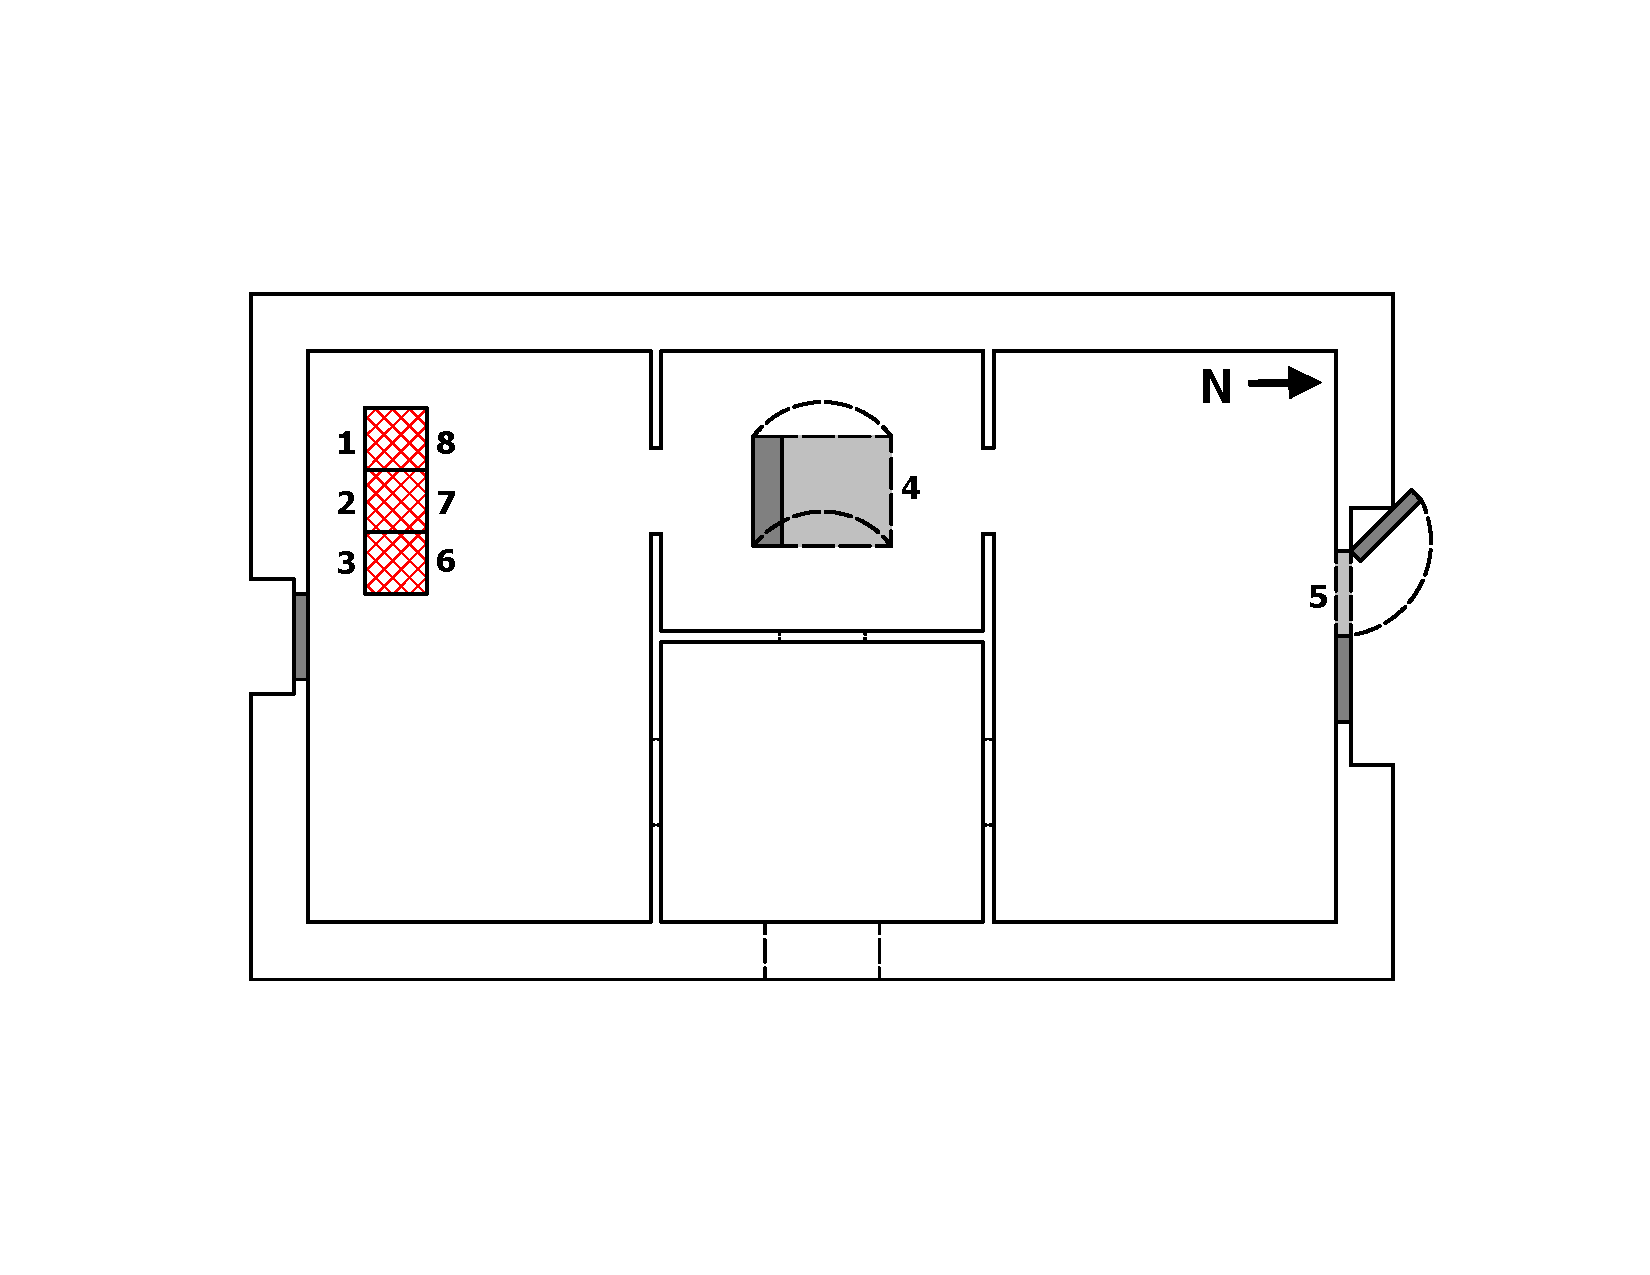
\includegraphics[width=\columnwidth]{../Figures/Floor_Plans/East_Structure_Test_6}
\end{minipage}
\caption{Test Series 6 layout and sequence of events.}
\label{fig:east_test_6}
\end{figure}
\FloatBarrier

\section{West Structure Tests}
Two different test series---Series 22 and Series 24---were conducted in the west structure. Each series was composed of two experiments that used an identical procedure to change the ventilation in the structure. Experiments conducted during Series 22 followed a procedure in which each double door on the first and second floors was opened. Experiments from Series 24 followed a sequence of events that involved opening the interior stairwell door, opening the west double door on both the first and second level, and opening the south side exterior door on the second level of the structure. Figs.~\ref{fig:west_test_22}~and~\ref{fig:west_test_24} include a schematic and additional details about the procedures used for the experiments during Series 22 and 24.

\begin{figure}[!ht]
\begin{minipage}[b]{0.8\columnwidth}
	\begin{flushleft}
	\small
	\begin{tabular}[b]{cc}
 	\toprule
 	\textbf{Number} & \textbf{Event Description} \\
 	\midrule
 	1-3  & Burners ignited \\
 	4	 & 2nd floor west double door opened \\
 	5 	 & 1st floor west double door opened \\
 	6	 & 2nd floor east double door opened \\
 	7 	 & 1st floor east double door opened \\
 	8-10  & Burners extinguished \\
	\bottomrule
	\end{tabular}
	\end{flushleft}
\end{minipage}
\begin{minipage}[b]{0.9\columnwidth}
	\vspace{15pt}
	\centering
	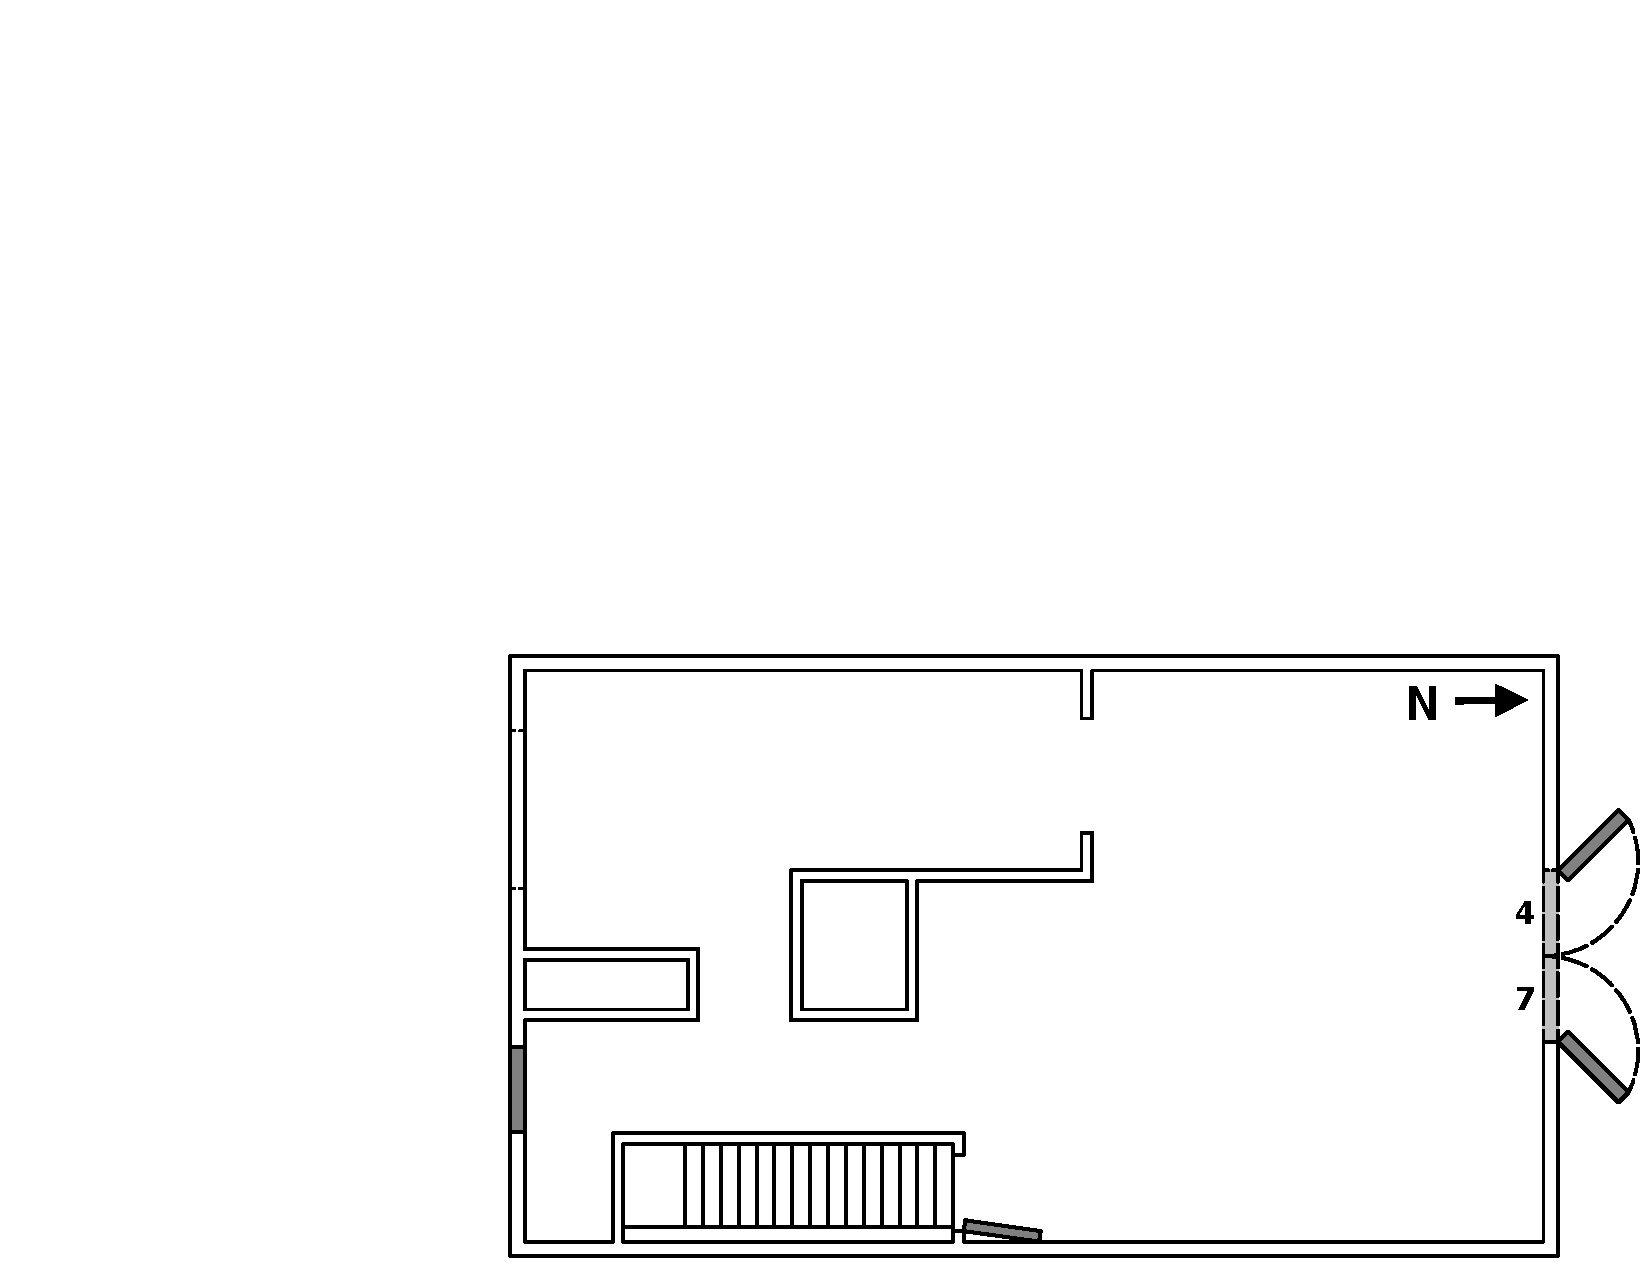
\includegraphics[width=\columnwidth]{../Figures/Floor_Plans/West_Structure_2nd_Floor_Test_22}
	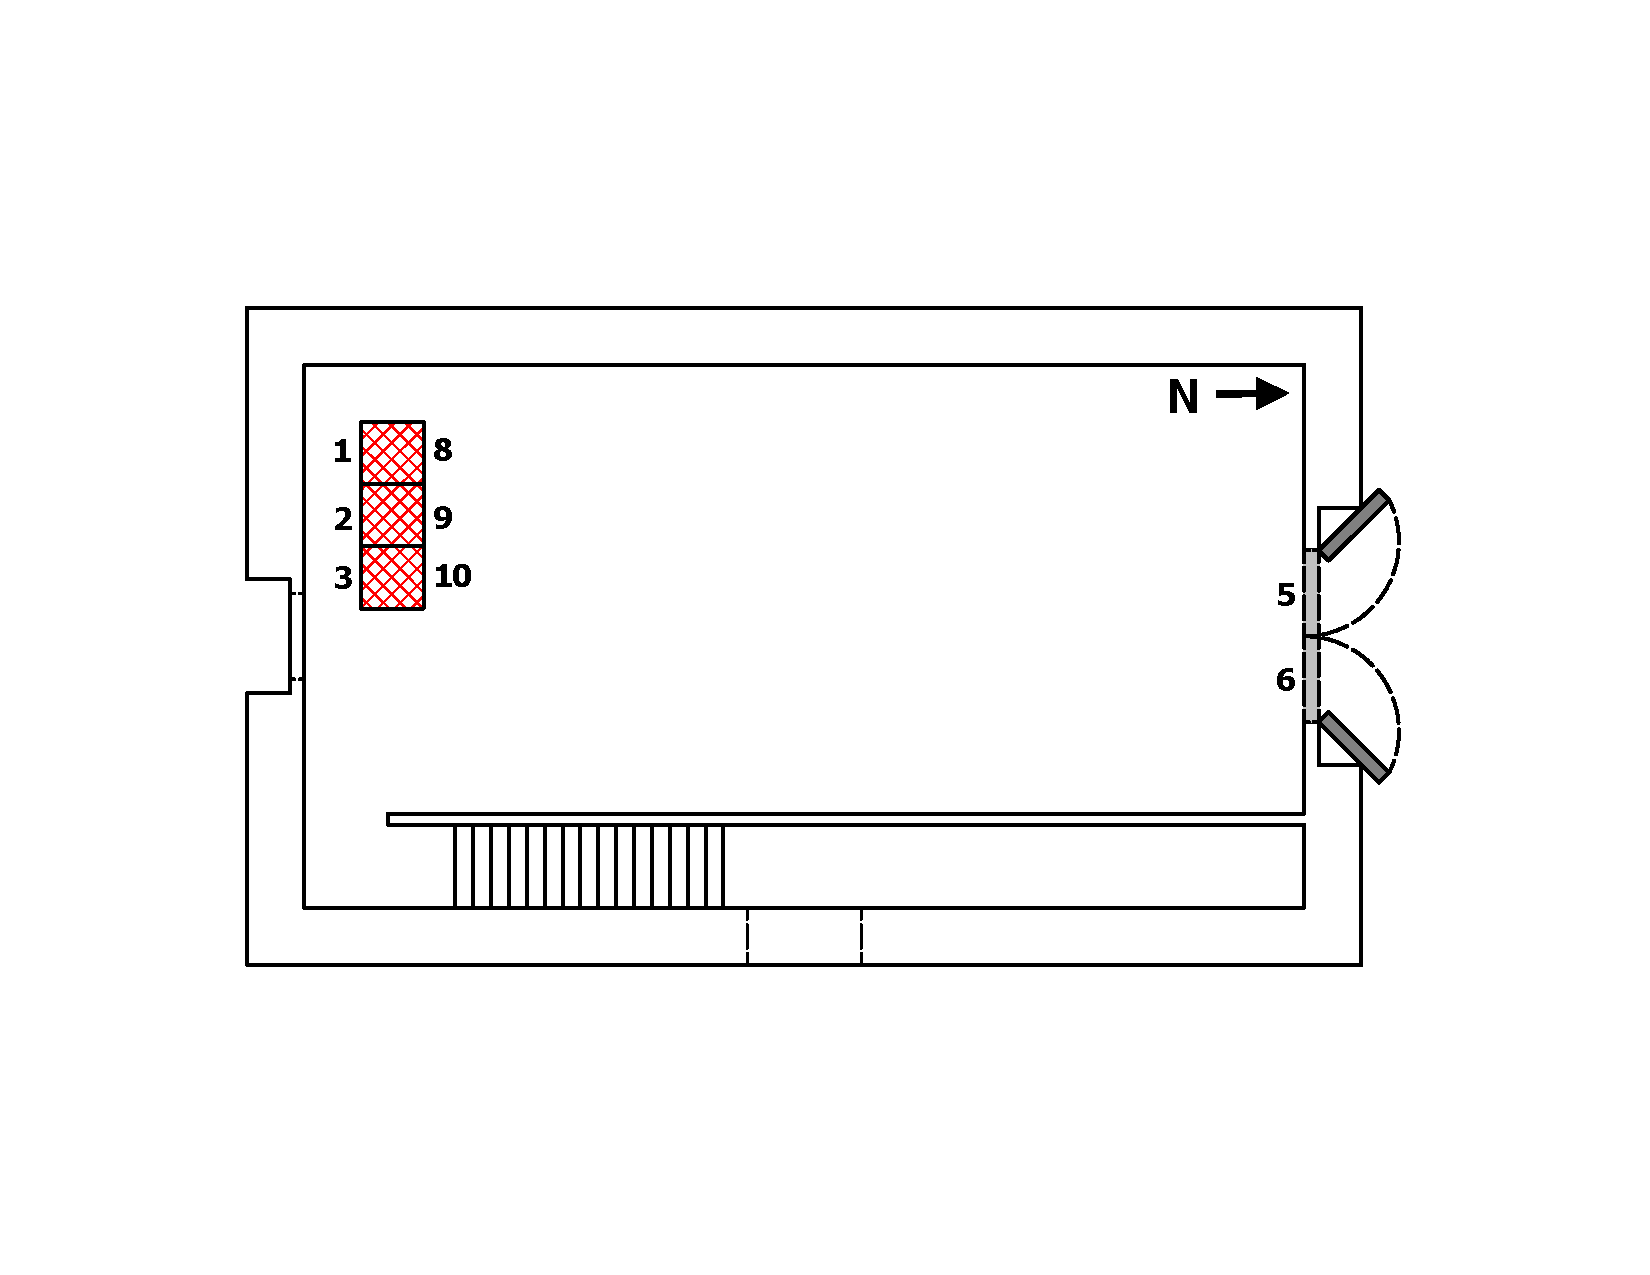
\includegraphics[width=\columnwidth]{../Figures/Floor_Plans/West_Structure_1st_Floor_Test_22}
\end{minipage}
\caption{Test Series 22 layout and sequence of events.}
\label{fig:west_test_22}
\end{figure}

\begin{figure}[!ht]
\begin{minipage}[b]{0.8\columnwidth}
	\begin{flushleft}
	\small
	\begin{tabular}[b]{cc}
 	\toprule
 	\textbf{Number} & \textbf{Event Description} \\
 	\midrule
 	1-3  & Burners ignited \\
 	4	 & Interior stairwell door opened \\
 	5 	 & 1st floor west double door opened \\
 	6	 & 2nd floor west double door opened \\
 	7 	 & 2nd floor south side door opened \\
 	8-10 & Burners extinguished \\
	\bottomrule
	\end{tabular}
	\end{flushleft}
\end{minipage}
\begin{minipage}[b]{0.9\columnwidth}
	\vspace{15pt}
	\centering
	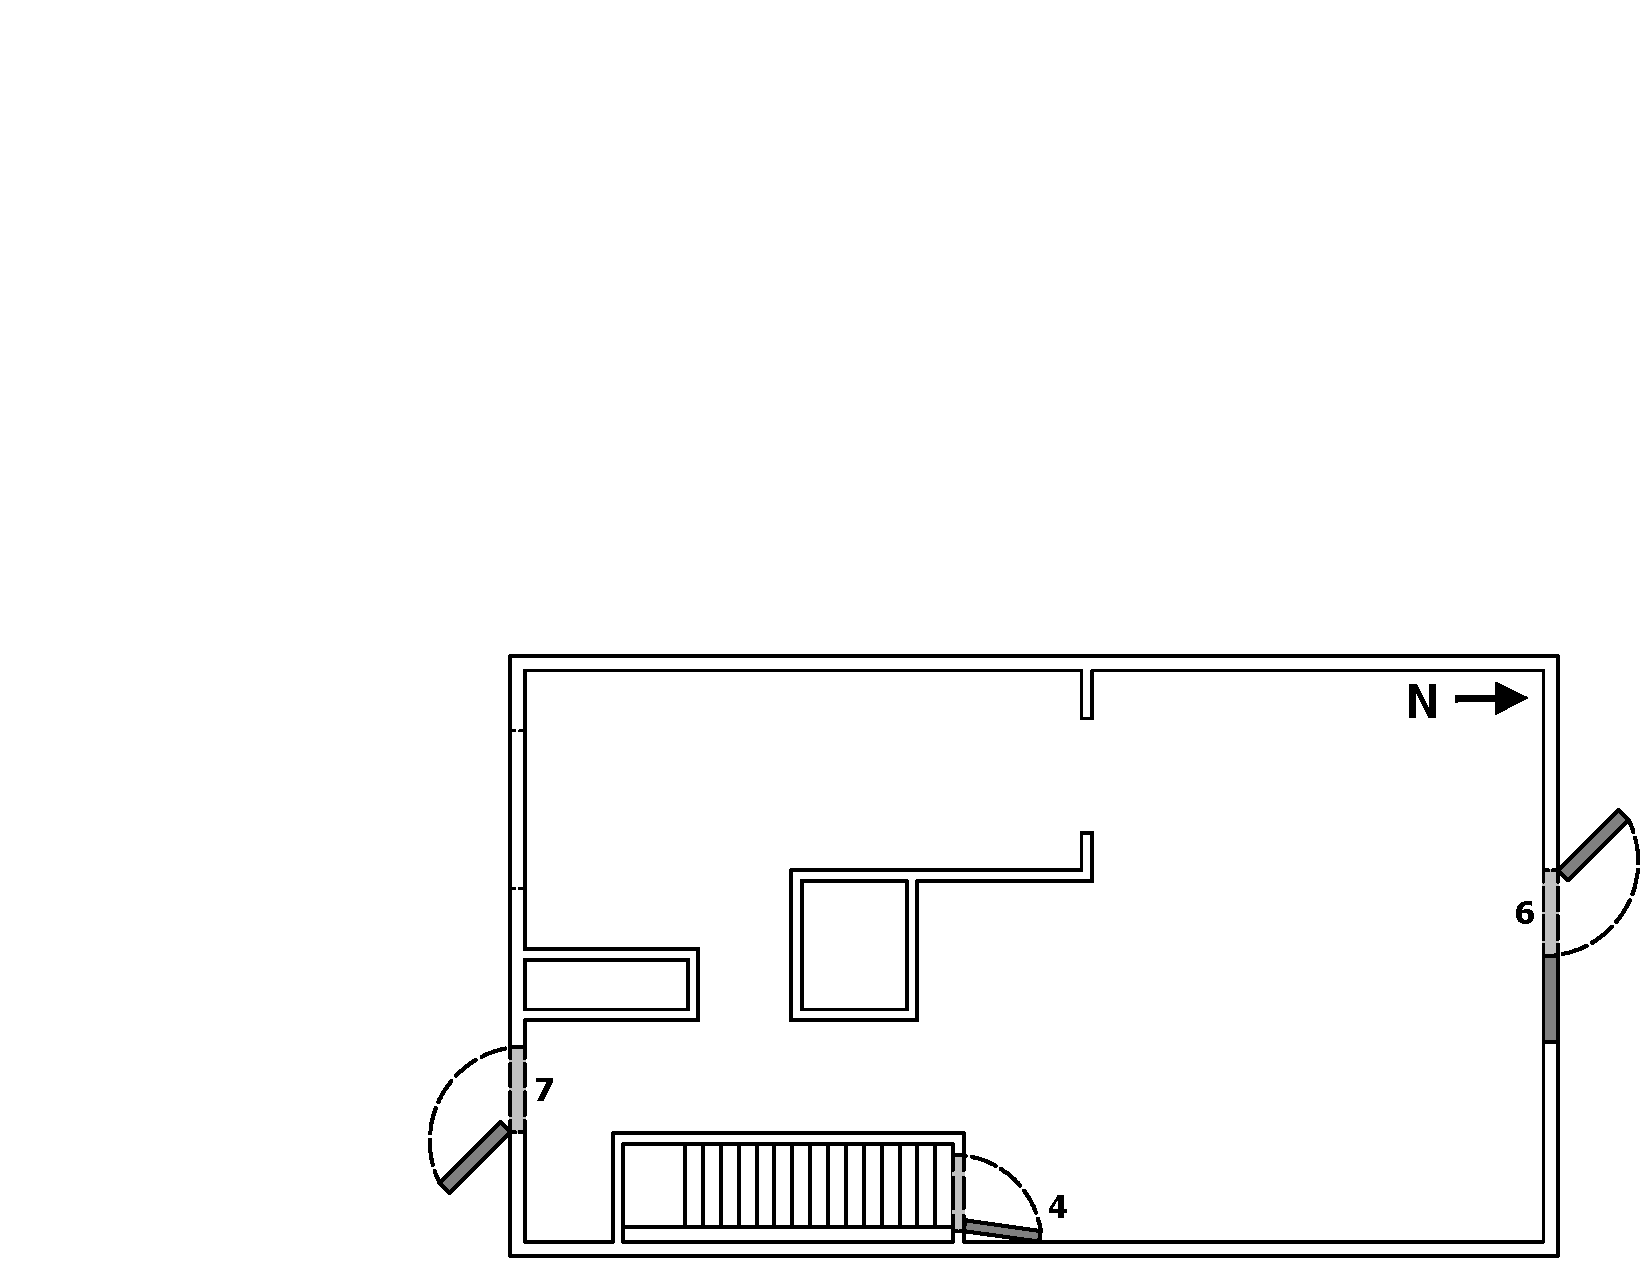
\includegraphics[width=\columnwidth]{../Figures/Floor_Plans/West_Structure_2nd_Floor_Test_24}
	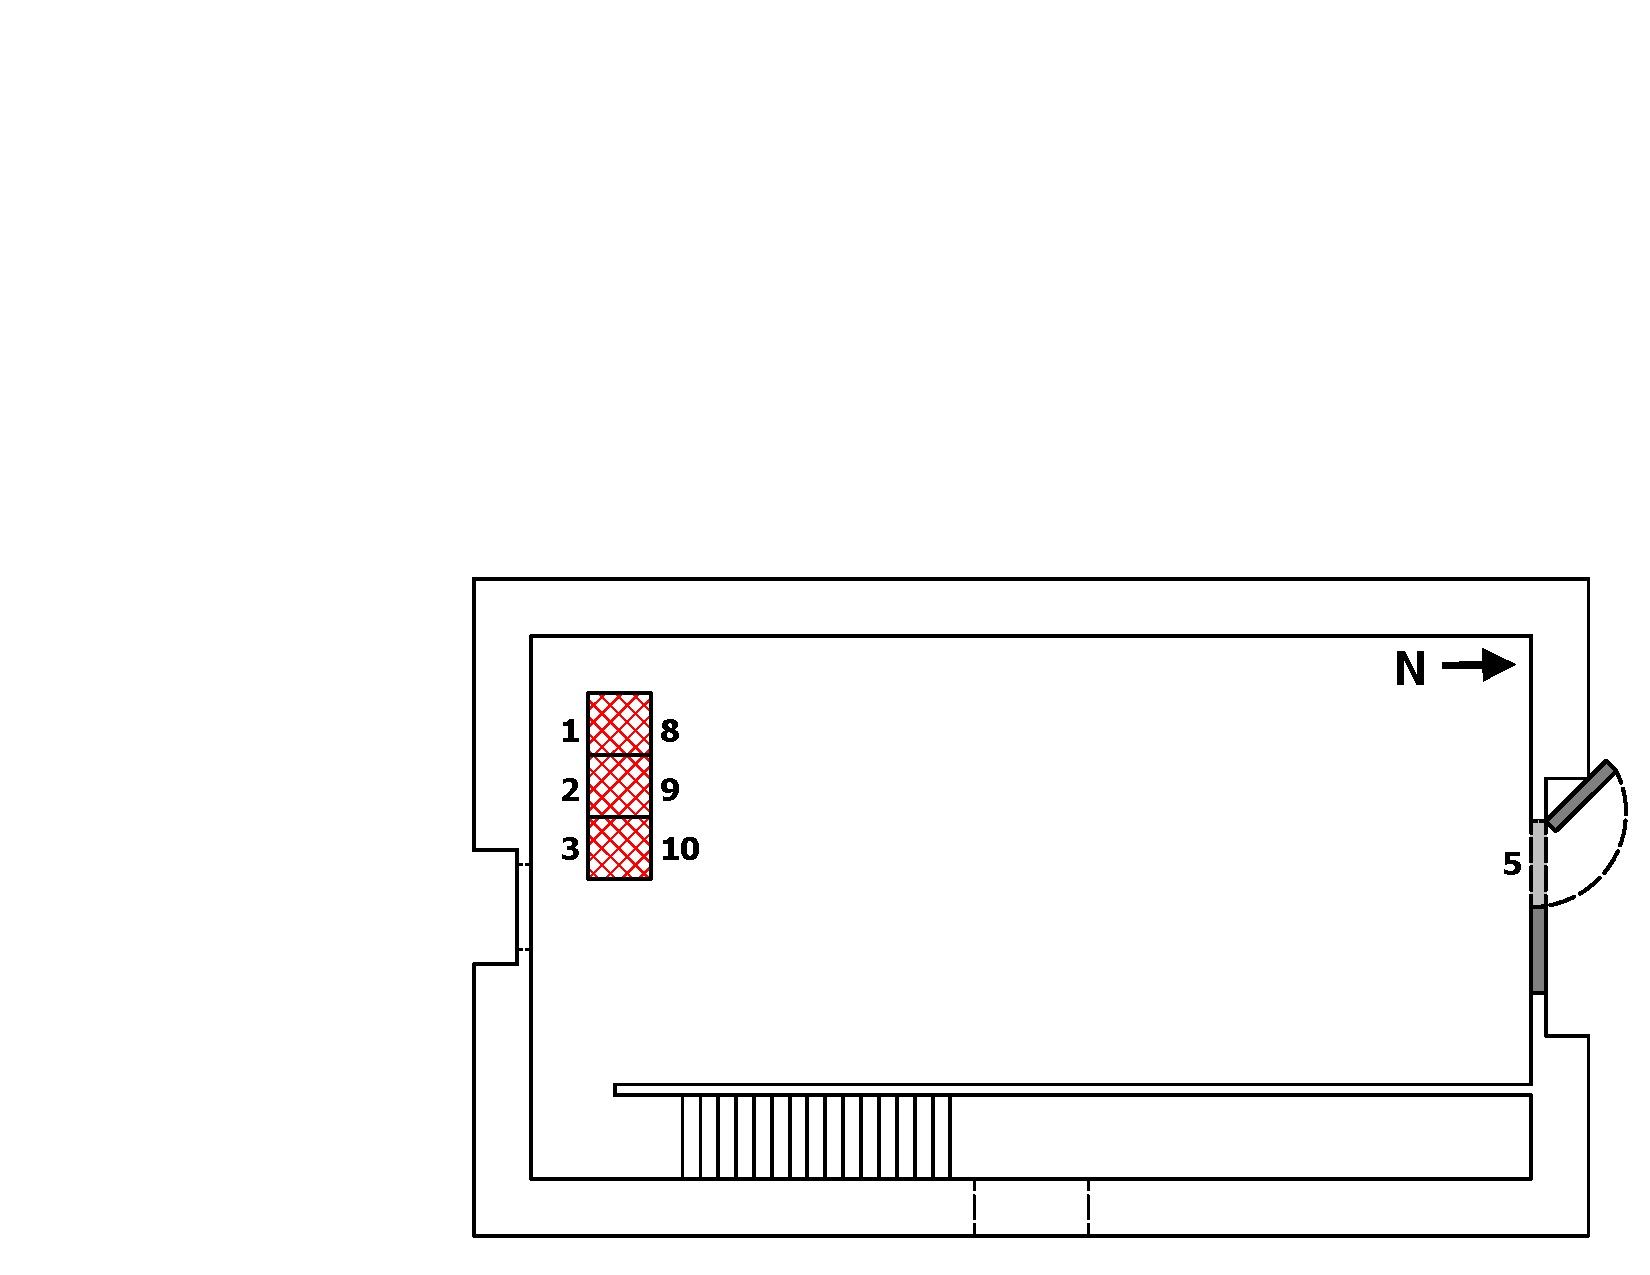
\includegraphics[width=\columnwidth]{../Figures/Floor_Plans/West_Structure_1st_Floor_Test_24}
\end{minipage}
\caption{Test Series 24 layout and sequence of events.}
\label{fig:west_test_24}
\end{figure}
\FloatBarrier

\chapter{Acknowledgments}
\label{chap:Acknowledgments}

\bibliography{../../../../../Bibliography/FDS_refs,../../../../../Bibliography/FDS_general}

\appendix

\chapter{Appendix A}

\begin{landscape}
\begin{table}[!ht]
\caption{East Structure experimental event times (mm:ss)}
\begin{tabular}{lcccccccccccccc}
 \toprule
\textbf{Test} & 
\multicolumn{2}{c}{\textbf{\underline{Corner Burner}}} & 
\multicolumn{2}{c}{\textbf{\underline{Middle Burner}}} & 
\multicolumn{2}{c}{\textbf{\underline{Center Burner}}} & 
\multicolumn{2}{c}{\textbf{\underline{W Double Door}}} & 
\multicolumn{2}{c}{\textbf{\underline{E Double Door}}} & 
\multicolumn{2}{c}{\textbf{\underline{Single Door}}} & 
\multicolumn{2}{c}{\textbf{\underline{Roof Vent}}}
\\
\textbf{Number} & 
\textbf{On} & \textbf{Off} & \textbf{On} & \textbf{Off} & \textbf{On} & \textbf{Off} & 
\textbf{Close} & \textbf{Open} & \textbf{Close} & \textbf{Open} &
\textbf{Close} & \textbf{Open} & \textbf{Close} & \textbf{Open}
\\
\midrule
% Test 2
2 & 0:20 & 16:20 & 3:20 & 14:20 & 6:20 & 12:20 & 
N/A & 7:20 & N/A & 9:20 & N/A & 10:30 & N/A & N/A \\
% Test 3
3 & 0:20 & 17:20 & 3:20 & 15:20 & 6:20 & 13:20 & 
N/A & 7:20 & N/A & 9:20 & N/A & 10:20 & N/A & N/A \\
% Test 4
4 & 0:20 & 17:20 & 3:20 & 15:20 & 6:20 & 13:20 & 
N/A & 7:20 & N/A & 9:20 & N/A & 10:20 & N/A & N/A 
\\ \multicolumn{15}{c}{ } \\
% Test 5a
5a & 0:15 & 9:55 & 0:30 & 9:35 & 0:45 & 9:15 & 
N/A & 3:18 & N/A & 6:18 & N/A & N/A & 7:45 & 2:53 \\
% Test 5b
5b & 0:15 & 10:30 & 0:30 & 10:15 & 0:45 & 10:00 & 
N/A & 3:45 & N/A & 5:15 & N/A & N/A & 8:30 & 2:15 \\
% Test 5c
5c & 0:15 & 9:45 & 0:30 & 9:30 & 0:45 & 9:15 & 
N/A & 3:45 & N/A & 5:16 & N/A & N/A & 7:28 & 2:15
\\ \multicolumn{15}{c}{ } \\
% Test 6a
6a & 0:15 & 9:55 & 0:30 & 9:35 & 0:45 & 9:15 & 
N/A & 3:18 & N/A & N/A & N/A & N/A & N/A & 2:53 \\
% Test 6b
6b & 0:15 & 9:55 & 0:30 & 9:35 & 0:45 & 9:15 & 
N/A & 3:18 & N/A & N/A & N/A & N/A & N/A & 2:53 \\
% Test 6c
6c & 0:15 & 9:55 & 0:30 & 9:35 & 0:45 & 9:15 & 
N/A & 3:18 & N/A & N/A & N/A & N/A & N/A & 2:53 \\
\bottomrule
\end{tabular}
\label{table:east_exp_times}
\end{table}
\end{landscape}


\end{document}
